\documentclass{article}

\usepackage{graphicx}
\usepackage{blindtext}
\usepackage{fancyhdr}
\usepackage{hyperref}

\usepackage[letterpaper, landscape]{geometry}

\geometry{tmargin=0.7in}
\geometry{bmargin=0.6in}

\geometry{lmargin=0.2in}
\geometry{rmargin=0.2in}

% ----------------

\newcommand{\hm}{\hspace*{1em}}
\newcommand{\hmm}{\hspace*{2em}}
\newcommand{\hmmm}{\hspace*{3em}}
\newcommand{\hmmmm}{\hspace*{4em}}

\newcommand{\ie}{\emph{i.e.,}}
\newcommand{\eg}{\emph{e.g.,}}
\newcommand{\etc}{\emph{etc.}}

% ----------------
% Set slide numbering to be on bottom left

\pagestyle{fancy}
\fancyhf{}

\lhead{\it Intro to RISC-V ISA}
\rhead{2022-12-06}

\lfoot{\footnotesize R.S.Nikhil}
\rfoot{\footnotesize Slide \thepage}

% ****************************************************************

\begin{document}

% ================================================================
% Title page

\vspace*{1in}

\begin{center}\Huge
  \emph{Introduction to the RISC-V ISA}

  \vspace*{0.5in}

  Rishiyur S. Nikhil \\
  December, 2022

  \vspace*{1in}

  
\includegraphics{Figs/Bluespec_Logo_2022-10.jpg}

  \vfill

  \begin{minipage}{7in}\Large
    {\bf Disclaimer:} any errors/opinions herein should be attributed
    only to the author and not to RISC-V International or to
    Bluespec, Inc.
  \end{minipage}

\end{center}

\clearpage

% ================================================================
% Contents

\begin{center}
  {\Huge Contents}

  \vspace{0.5in}

  \begin{minipage}{9in}\LARGE
    \begin{itemize}

    \item RISC-V: general information

    \item RISC-V ISA's modular organization
      \begin{itemize}
      \item I(nteger) + optional extensions M, A, F, D, C, ...
      \item Unprivileged and Privileged
      \end{itemize}

    \item Unprivileged ISA overview (I, M, A, F, D, C)

    \item Memory and I/O

    \item Privileged ISA
      \begin{itemize}
      \item CSRs (Control and Status registers)
      \item Exceptions (traps and interrupts)
      \item Supervisor privilege level and Virtual Memory
      \end{itemize}

    \item Common artefacts attached to cores:
      \begin{itemize}
      \item CLIC: software interrupts, real-time timer, timer interrupts
      \item PLIC: Platform-Level Interrupt controller
      \item Debug Module
      \end{itemize}

    \item Comments on software for RISC-V
    \end{itemize}
  \end{minipage}
\end{center}

\clearpage

% ================================================================
% References

\begin{center}\LARGE
  {\Huge Primary References}

  \vspace{0.5in}

  \begin{minipage}{9in}
    Unprivileged and Privileged ISAs:

    \begin{itemize}
    \item \emph{The RISC-V Instruction Set Manual; Volume I:
    Unprivileged ISA, Document Version 20191213}, Andrew Waterman and
      Krste Asanović (editors), December 13, 2019, 238 pp.

    \item \emph{The RISC-V Instruction Set Manual; Volume II: Privileged Architecture,
    Document Version 20211203}, Andrew Waterman, Krste Asanović1 and John Hauser (editors)
      December 4, 2021, 155 pp.
    \end{itemize}

    \vspace{1in}

    PDFs for all RISC-V specs can be found at: \\
    \hmmmm \url{https://riscv.org/technical/specifications/}
  \end{minipage}

  \vfill

  Note: ARM’s 64-bit architecture (ARM v8-A) spec is over 6000 pages long.

\end{center}

\clearpage

% ================================================================
% "RISC-V" is only an ISA

\begin{figure}[htp]
    \centering
    {\Huge ``RISC-V'', per se, is \emph{only} an ISA (Instruction Set Architecture)}

    \vspace{0.5in}

    \begin{minipage}{9in}\LARGE
      \begin{itemize}
      \item Only a specification, a document, describing:
        \begin{itemize}
        \item ``Architecturally-visible'' state: registers (PC, integer, PC, floating point, CSRs)
        \item Repertoire of instructions, and binary representation of each one
        \item Semantics (meaning) of each instruction: how it
          accesses/changes architecturally visible state
        \end{itemize}
        {\ie} it's the abstract view of the machine targeted by general-purpose compilers.

      \item Not an actual CPU, processor, chip, core, ...

      \item \emph{Not within the purview of the ISA}:
        micro-architectural choices in particular implementations,
        such as pipeline structure, instruction pre-fetch,
        branch-prediction and other speculation, bypassing,
        superscalarity, out-of-order execution, multithreading,
        caches, MHz, CPI, energy consumption, {\etc}

        There can be a variety of implementations varying widely on
        these dimensions, from IoT microcontrollers to server-class
        cores to supercomputing cores.

      \end{itemize}
    \end{minipage}
\end{figure}

\clearpage

% ================================================================
% RISC-V is an open ISA

\begin{figure}[htp]
    \centering
    {\Huge RISC-V is an \emph{Open} ISA, unlike other ISAs}

    \vspace{0.5in}

    \begin{minipage}{9in}\LARGE
      \begin{itemize}

        \item There are many well-known, mature ISAs---x86, ARMv8,
          Power, Sparc, ...---but they are all \emph{proprietary},
          requiring licenses and fees if you want to implement them.

        \item RISC-V does not require any license fee to
          implement.$^1$

          \begin{itemize}
          \item This is central to all the current commercial interest in RISC-V.
          \item This is central to \emph{architecture researchers} who
            wish to innovate on state-of-the-art implementations, and
            indeed was the original motivation behind the creation of
            RISC-V by a team at Univ. of California, Berkeley.
          \end{itemize}

        \item RISC-V seems well on its way to becoming one of the
          three dominant ISAs (along with x86 and ARM).
      \end{itemize}
    \end{minipage}
\end{figure}

\vfill

{$^1$ The name ``RISC-V'' is owned by RISC-V International, and you
  need their permission to use the name in commercial naming of
  products.}

\clearpage

% ================================================================
% The RISC-V ISA has a Modular Organization

\begin{center}
{\Huge
  The RISC-V ISA has a \emph{Modular} Organization}

\vspace*{0.3in}

{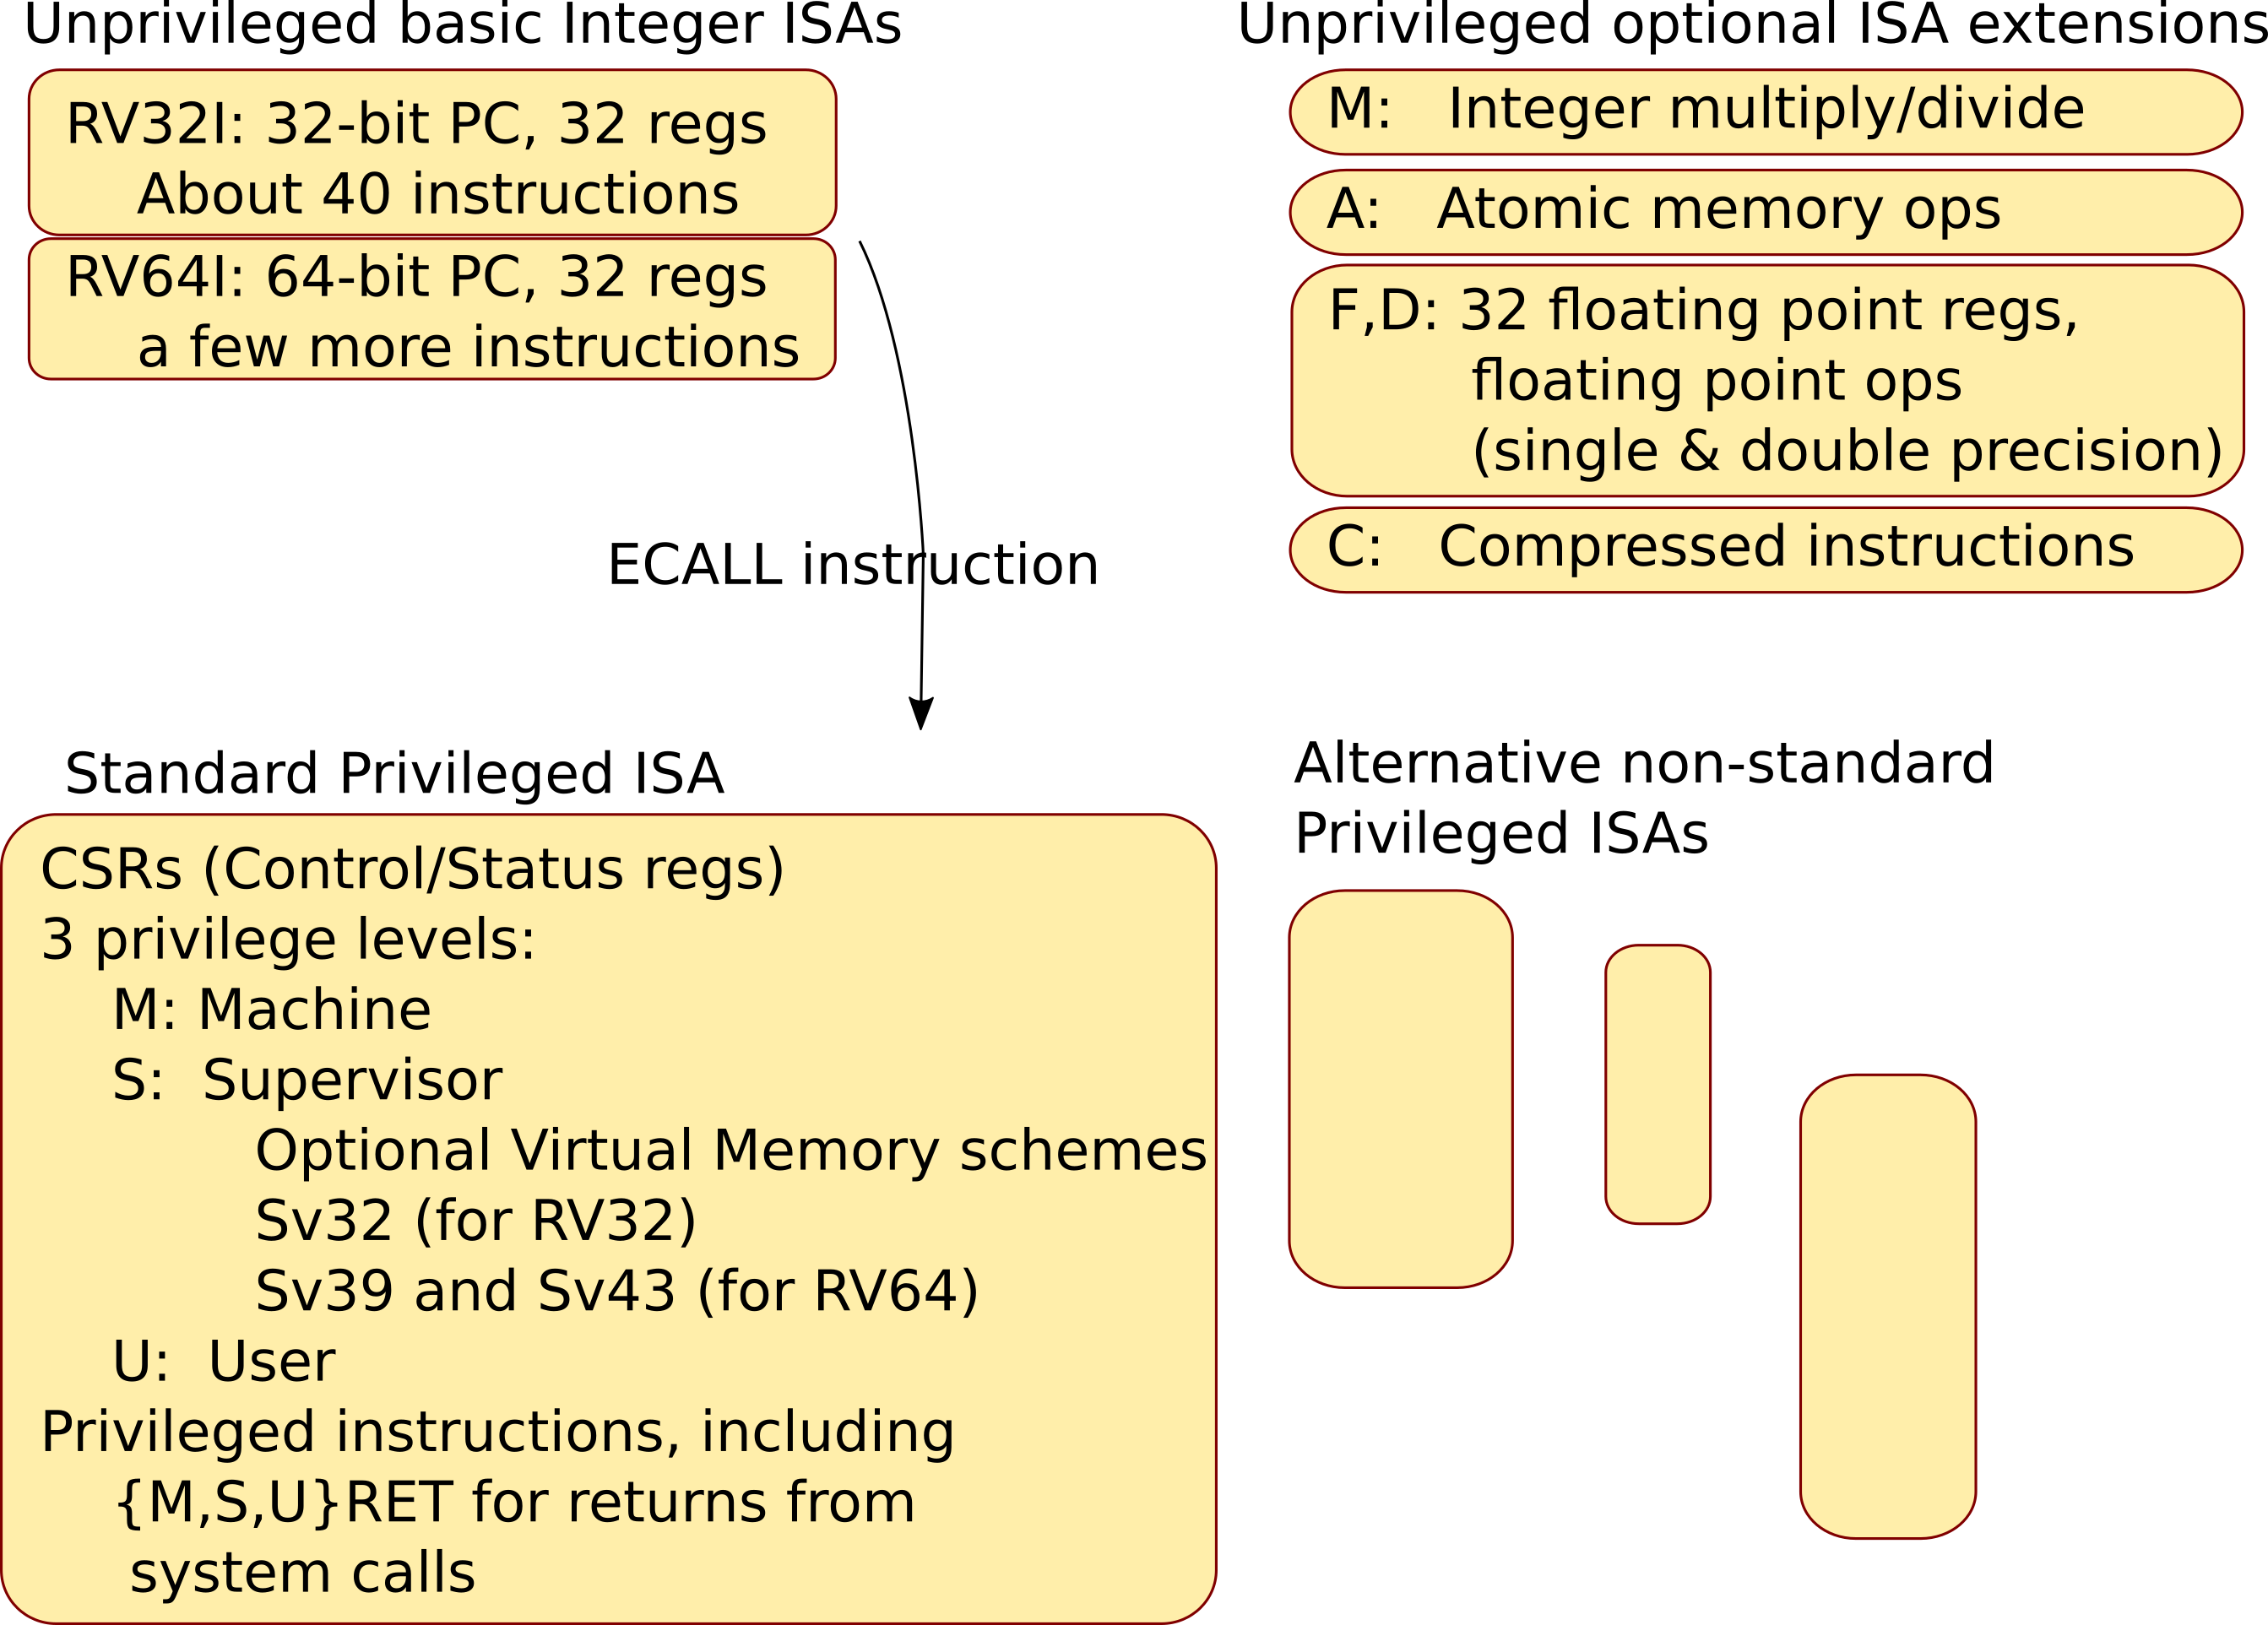
\includegraphics[scale=0.7]{Figs/ISA_Modularity.png}}

PDFs for all RISC-V specs can be found at: \url{https://riscv.org/technical/specifications/}

\begin{itemize}\LARGE

\item Many other standard extensions exist: vector, crypto, bit-manipulation, ...

\item Implementors can choose according to target, from small
  IoT/Embedded ({\eg} RV32IC ``bare-metal'') to server-class/HPC (e.g.,
  RV64IMAFDC with vector, crypto, bit-manipulation and standard
  Privileged ISA)

\item HW facilities allow SW to discover the configuration on which it is running.

\end{itemize}

\end{center}

\clearpage

% ================================================================
% Instruction formats

\begin{center}
{\Huge
  Instruction formats}

\vspace{1ex}

PDFs for RISC-V specs can be found at: \url{https://riscv.org/technical/specifications/}

\begin{itemize}\LARGE
\item All instructions are 32-bits wide, for both RV32 and RV64.

\item  There are very few instruction formats (simplifies hardware-decoder in CPU pipelines).
\end{itemize}

\vspace{0.5in}

\fbox{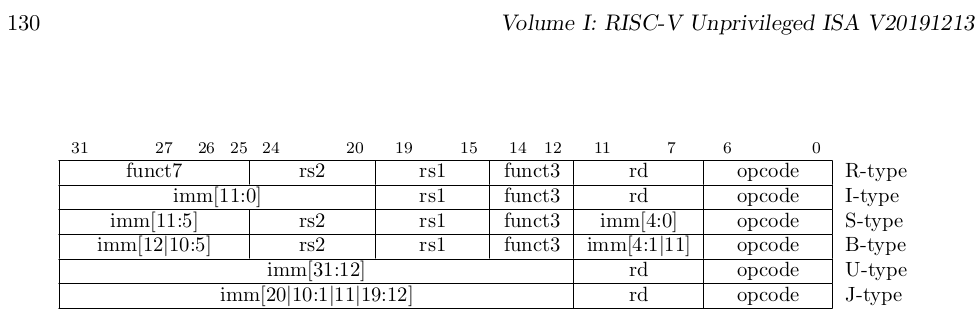
\includegraphics[height=3.25in]{Figs/UNPRIV_riscv-spec-20191213_p130_Instr_Formats.png}}

\vspace{0.5in}

\begin{itemize}\LARGE
\item In the optional ``C'' extension (``compressed''), instructions
  are 16-bits wide, for small-footprint systems (IoT/Embedded/Edge).

\item Each 16-bit C instruction expands to a standard 32-bit RV32/64
  instruction; so only needs hardware at the front-end of the CPU
  pipeline (16-bit fetch and expansion).
\end{itemize}

\end{center}

\clearpage

% ================================================================
% Basic integer instruction set

\begin{center}
{\Huge
  Base Unpriviliged Integer ISA (with 32 32-bit or 64-bit registers)}

\vspace*{1ex}

PDFs for RISC-V specs can be found at: \url{https://riscv.org/technical/specifications/}

\vspace*{1ex}

\vfill

\begin{minipage}[t]{5in}
  \hmm \\
  \fbox{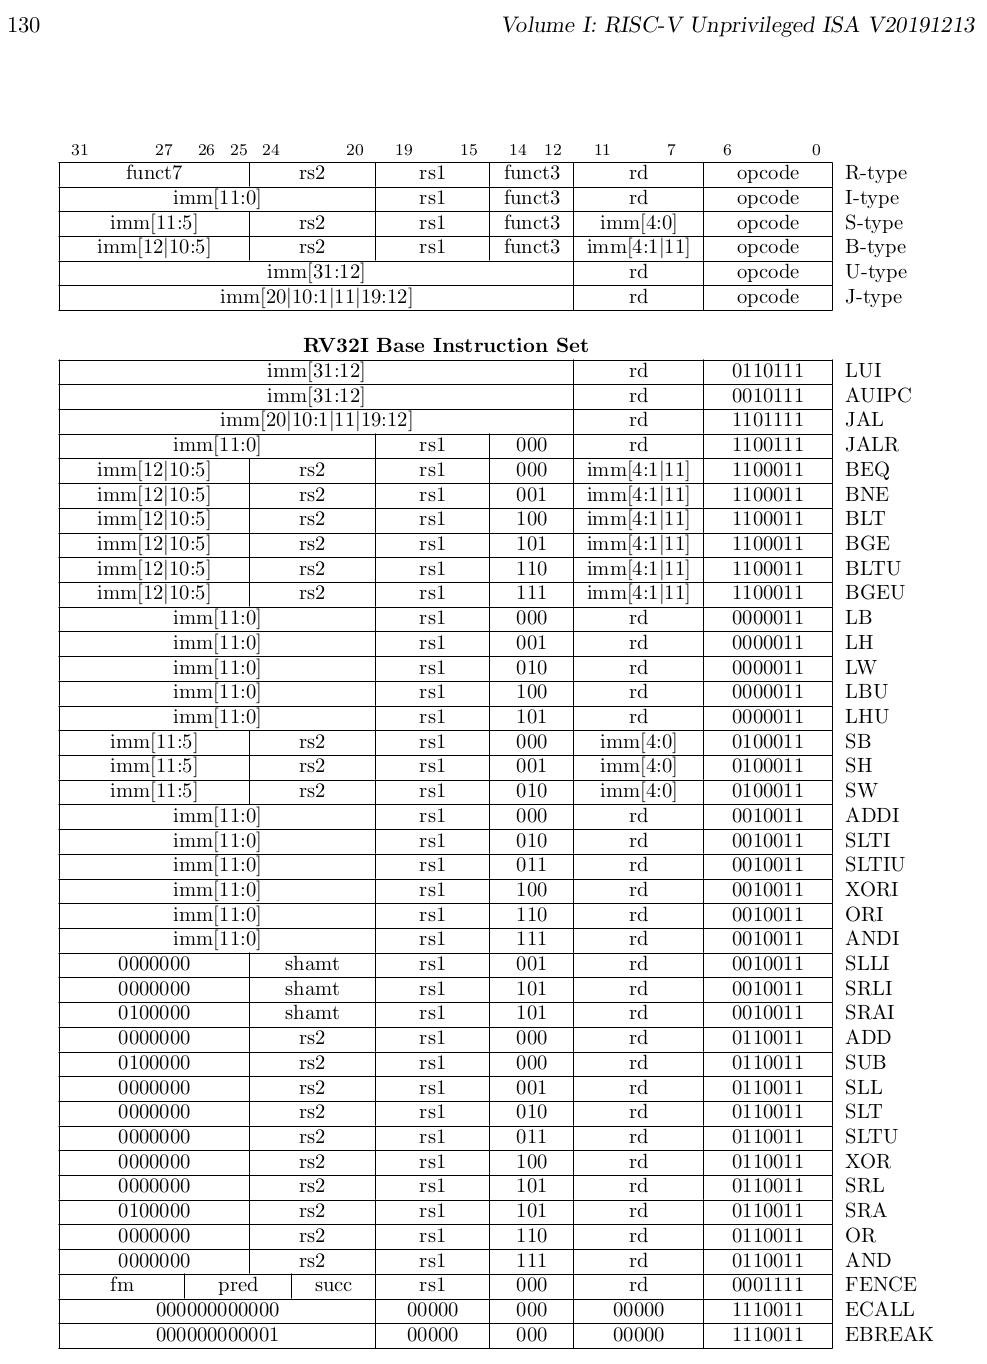
\includegraphics[width=4.5in]{Figs/UNPRIV_riscv-spec-20191213_p130_RV32I.png}}
\end{minipage}
\hm
\begin{minipage}[t]{5in}
  \hmm \\
  \begin{itemize}\large

  \item RV32I ISA (Unprivileged, 32 x 32-bit registers, integer only)
    has a mere 40 instructions (left)

  \item RV64I ISA (32 x 64-bit registers) adds 15 more instructions
    (below)

  \end{itemize}

  \vspace{0.1in}

  \fbox{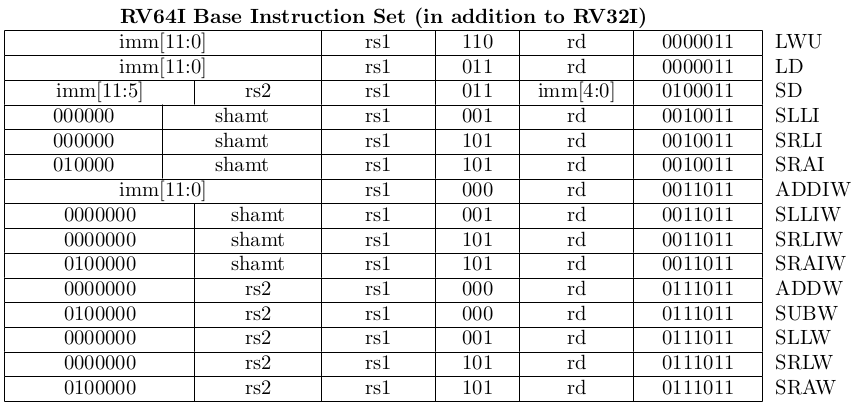
\includegraphics[width=4.5in]{Figs/UNPRIV_riscv-spec-20191213_p131_RV64I.png}}

  \begin{itemize}\large

  \item AUIPC (Add Upper Immediate to PC): enables position-independent code.

  \item Pure ``Load-Store'' ISA, {\ie} complete separation of memory
    access instructions from all other instructions (Lx, Sx).

  \item All I/O is via memory-mapped registers; no separate instructions.

  \item ECALL: ``call-out'' to Privileged ISA.  Details are part of
    Privileged Spec.

  \item EBREAK: ``call-out'' to debugging environment (unspecified).

  \end{itemize}
  {\large \emph{Possibly the cleanest, most orthogonal, industrial-strength ISA ever.}}
\end{minipage}

\end{center}

\clearpage

% ================================================================
% Integer Multiply/Divide

\begin{center}
  {\Huge
    ``M'' extension: Integer Multiply and Divide instructions}

  \vspace*{0.5in}

  \fbox{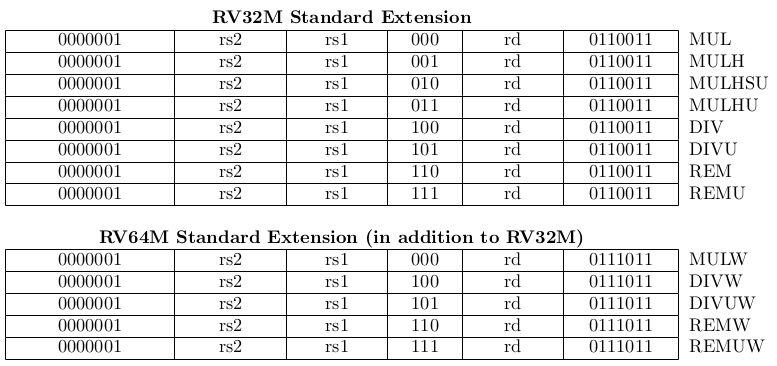
\includegraphics[width=7in]{Figs/UNPRIV_riscv-spec-20191213_p131_M.png}}

  \vspace{0.2in}

  \begin{minipage}{7in}\large
    \begin{itemize}

      \item S: signed; U: Unsigned:
        enables signed and unsigned multiplications.

      \item H: upper half of double-width data: enables 64-bit
        multiplications on RV32, 128-bit multiplications on RV64.

      \item W: enables 32-bit multiplications on RV64.

    \end{itemize}
  \end{minipage}
\end{center}

\clearpage

% ================================================================
% Atomic mem ops

\begin{center}
  {\Huge
    ``A'' extension: Atomic memory operations}

  \vspace{0.2in}

  \fbox{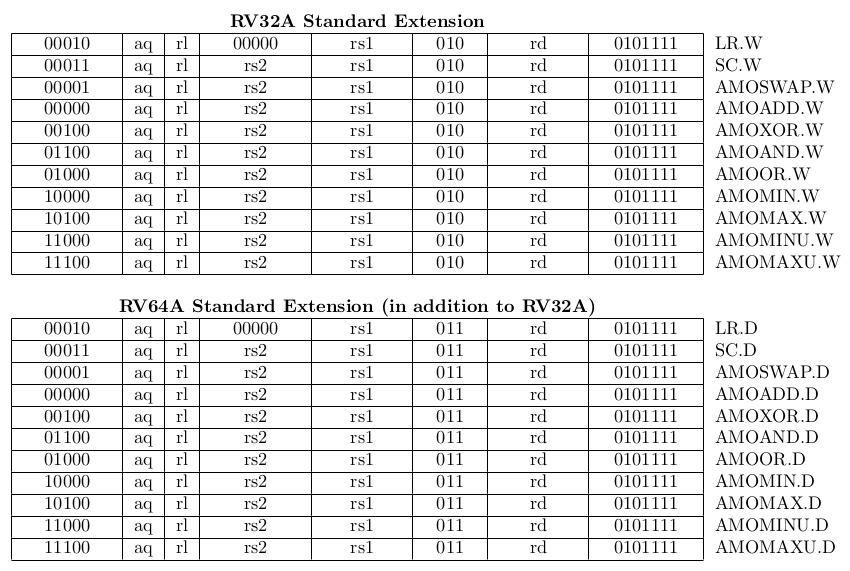
\includegraphics[width=7in]{Figs/UNPRIV_riscv-spec-20191213_p132_A.png}}

  \vspace{0.2in}

  \begin{minipage}[t]{6in}
    \begin{itemize}\Large
    \item LR/SC: ``Load Reserved/Store Conditional'' on a memory location
    \item AMOxxx: atomic read-modify-writes on a memory location
    \item W ops operate on aligned 32-bit words
    \item D ops operate on aligned 64-bit words
    \end{itemize}
  \end{minipage}
\end{center}

\clearpage

% ================================================================
% Atomic mem ops

\begin{center}
  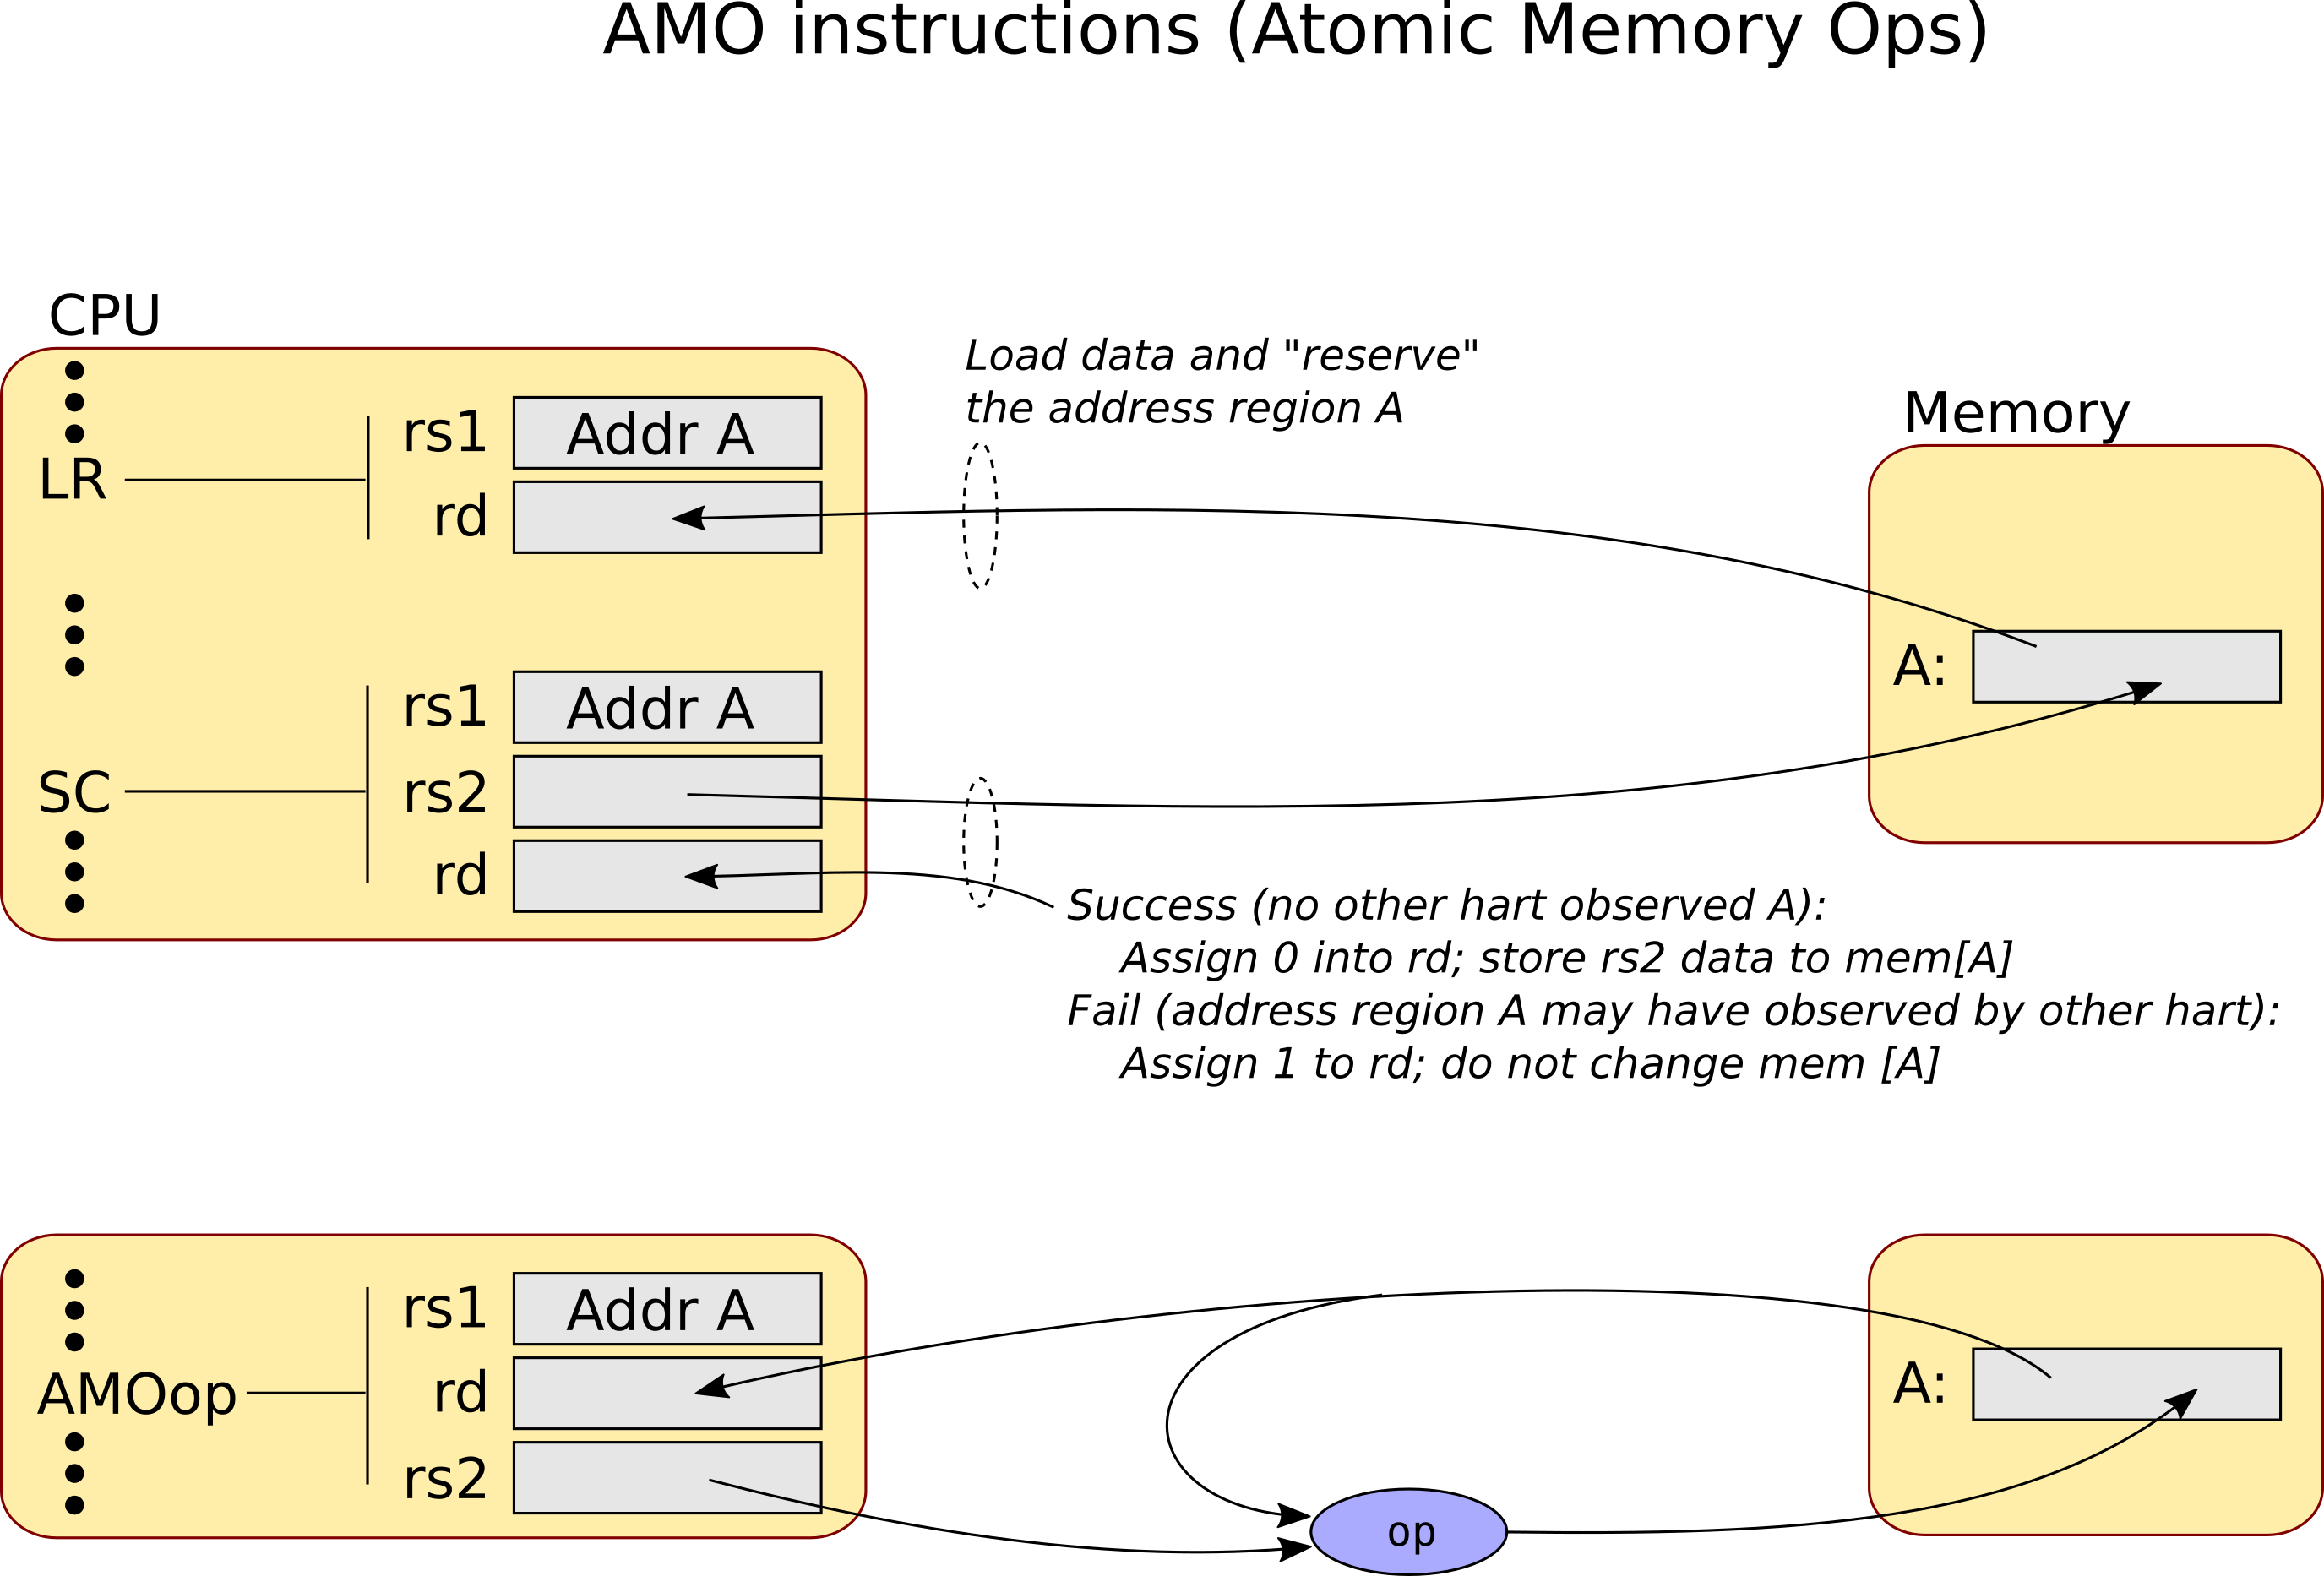
\includegraphics[width=7in]{Figs/LR_SC_AMO.png}

  \vspace{1in}

  \begin{minipage}[t]{8in}
    \begin{itemize}\Large
    \item LR/SC: Typically in a loop, until success

    \item LR/SC: Many nuances on ``address region'', ``observed by
      another hart'', number and type of instructions between the LR
      and SC, ...
    \end{itemize}

    \vspace*{5ex}

    {\large $^*$ ``hart'' $=$ ``hardware thread'', a single hardware
      thread, based on a single instruction-fetch unit}
  \end{minipage}
\end{center}


\clearpage

% ================================================================
% Single-precision Floating point

\begin{center}
{\Huge
  ``F'' extension: IEEE Single-precision Floating Point}
\end{center}

\vspace*{0.1in}

{\LARGE State: 32 x 32-bit floating-point registers, plus these CSRs (Control/Status Regs)}

\begin{center}
  \fbox{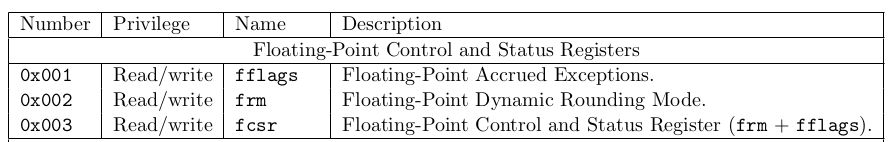
\includegraphics[width=7in]{Figs/UNPRIV_riscv-spec-20191213_p136_CSRs_FD.png}}
\end{center}

\vspace*{0.1in}

{\LARGE Instructions:}

\begin{center}
  \fbox{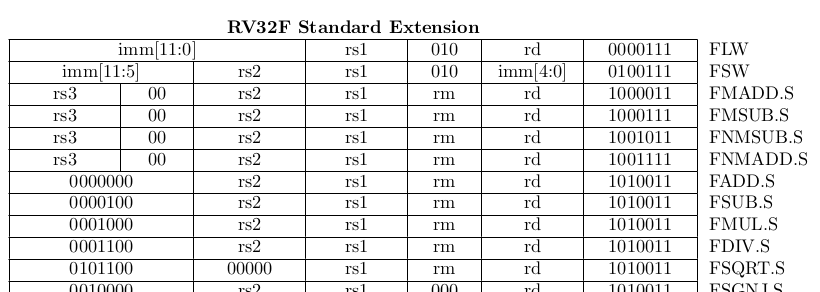
\includegraphics[width=7in]{Figs/UNPRIV_riscv-spec-20191213_p133_RV32F.png}}

  \vspace*{1ex}

  {\Large (... more ... please consult spec)}
  \vspace*{0.2in}

  \fbox{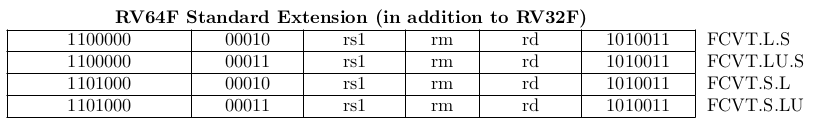
\includegraphics[width=7in]{Figs/UNPRIV_riscv-spec-20191213_p133_RV64F.png}}
\end{center}

\clearpage

% ================================================================
% Double-precision Floating point

\begin{center}
{\Huge
  ``D'' extension: IEEE Double-precision Floating Point}
\end{center}

\vspace*{0.1in}

{\LARGE 32 x 64-bit floating-point registers, plus these CSRs (Control/Status Regs)}

\begin{center}
  \fbox{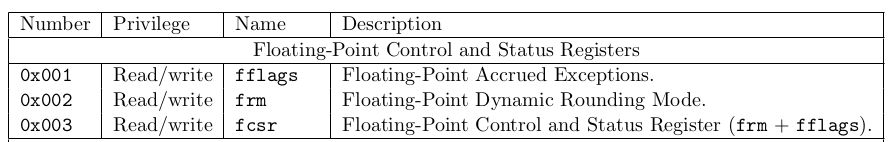
\includegraphics[width=7in]{Figs/UNPRIV_riscv-spec-20191213_p136_CSRs_FD.png}}
\end{center}

\vspace*{0.1in}

{\LARGE Instructions:}

\begin{center}
  \fbox{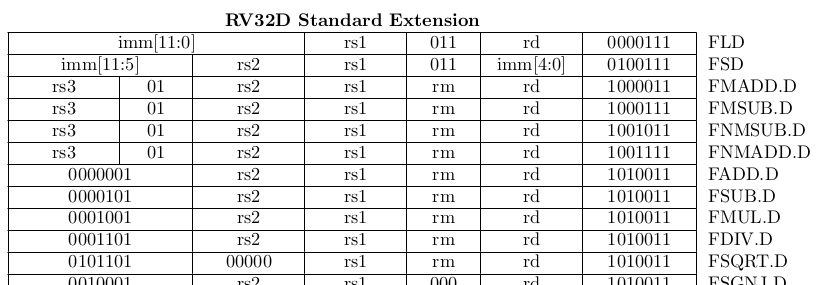
\includegraphics[width=7in]{Figs/UNPRIV_riscv-spec-20191213_p134_RV32D.png}}

  \vspace*{1ex}

  {\Large (... more ... please consult spec)}

  \vspace*{0.2in}

  \fbox{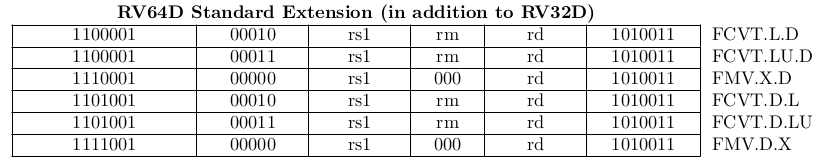
\includegraphics[width=7in]{Figs/UNPRIV_riscv-spec-20191213_p134_RV64D.png}}
\end{center}

\clearpage

% ================================================================
% Compressed Instructions

\begin{center}
  {\Huge
    ``C'' extension: Compressed Instructions for smaller footprint}

  \vspace*{0.2in}

  \fbox{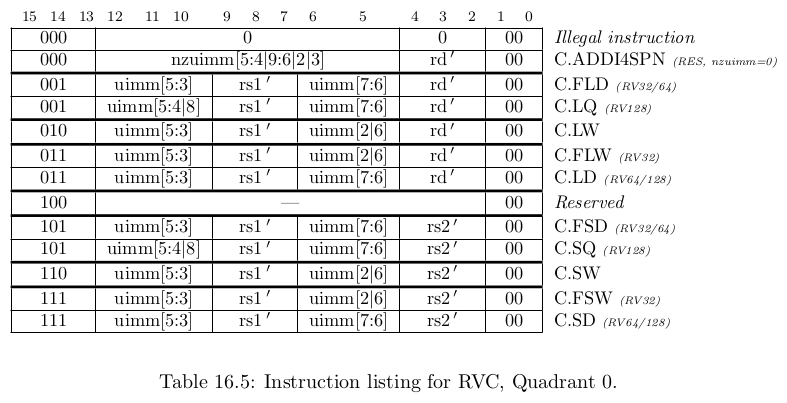
\includegraphics[width=7in]{Figs/UNPRIV_riscv-spec-20191213_p112_RVC_Q0.png}}
                                    

  \vspace*{0.1in}

  {\Large (... more ... please consult spec)}

  \vspace*{0.3in}

  \begin{minipage}{9in}\LARGE
    \begin{itemize}
    \item ``C'' instructions are 16-bits wide, can be packed two-to-a-32b-word.

    \item Not standalone; are mixed with standard 32-bit instructions.

    \item 3-bit register fields refer to the 8 ``most popular'' registers.

    \item Each 16-bit C instruction expands to a standard 32-bit RV32/64
      instruction; so only needs hardware at the front-end of the CPU
      pipeline (16-bit fetch and expansion).

    \item Include M, F, D instructions.
    \end{itemize}
  \end{minipage}
\end{center}

\clearpage

% ================================================================
% Memory and I/O

\begin{center}
  {\Huge
    Notes on Memory and I/O}

  \vspace*{0.5in}

  \begin{minipage}{9in}\LARGE
    \begin{itemize}

    \item Pure ``Load-Store'' ISA (with register base-address +
      index), {\ie} total separation of memory instructions
      vs. non-memory instructions.

    \item Flat memory space (address-width depends on RV32 or RV64, and Virtual Memory Scheme).

    \item All I/O through memory-mapped device registers; no separate I/O instructions.

    \item Optional PMP CSRs (Physical Memory Protection) can impose
      base-and-bounds regions on memory with access permissions.  This
      provides lightweight sandboxing without the overheads of full
      Virtual Memory (MMUs, page tables, address translation, ...).

    \item FENCE, FENCE.I, and SFENCE.VMA instructions for
      implementations that need to synchronize multicores, I-Caches
      and D-Caches, and MMUs with Caches.

    \item For multicores, RISC-V has an ARM-like ``Weak Memory
      Model'', enabling more re-ordering of memory traffic for higher
      performance.  Also has a a TSO option, which is a stricter
      memory model (like x86).

    \end{itemize}
  \end{minipage}
\end{center}

\clearpage

% ================================================================
% Privileged ISA

\begin{center}
  {\Huge
    Standard Privileged ISA}

  \vspace*{0.5in}

  \begin{minipage}{9in}\LARGE
    {\Large Note: The separation between Unprivileged and Privileged ISAs is very
    clean.  A CPU implementation can easily implement a non-standard
    Privileged ISA with the standard Unprivileged ISA, if desired.}

    \vspace{0.5in}

    Privilege Levels: enables clean \emph{virtualization} (hypervisors, Xen, VMWare, ...)

    \begin{center}
      \begin{tabular}{|c|c|l|c|}
        \hline
        Level & Code & Name                 & Comment \\
        \hline
        3     & 11   & M (Machine)          & Highest privilege; firmware, boot loaders, ... \\
        2     & 10   & \hmm \emph{Reserved} & \\
        1     & 01   & S (Supervisor)       & Operating systems (like Linux) \\
        0     & 00   & U (User/Application) & Applications \\
        \hline
      \end{tabular}
    \end{center}

    \vspace{0.5in}

    Implementations do not have to implement all privilege levels
    (implementation cost tradeoff):

    \begin{center}
      \begin{tabular}{|c|c|}
        \hline
        Implemented Levels & Intended Usage \\
        \hline
        M                  &   Simple embedded systems (``bare metal'') \\
        M,U                &   Secure embedded systems \\
        M,S,U              &   Full OS + apps \\
        \hline
      \end{tabular}
    \end{center}
  \end{minipage}

\end{center}

\clearpage

% ================================================================
% Privileged ISA

\begin{center}
  {\Huge
    Standard Privileged ISA: CSRs (Control and Status Registers)}

  \vspace*{0.2in}

  \begin{minipage}{9.5in}\Large
    \begin{itemize}

      \item CSRs: additional set of registers in the CPU, identified
        by 12-bit CSR number.

      \item Up to 4096 possible CSRs, but most are optional; only a
        small handful are essential in an implementation.

      \item CSRs can be accessed programmatically with the CSR
        instructions shown below, each of which atomically swaps the
        contents of a CSR with standard integer registers, with some
        variations and nuances.

      \item CSR instructions can be used at all privilege levels, but
        the upper 4 bits of a CSR's number specifies which privilege
        levels can access that particular CSR, and with which
        ops (read, read/write).

      \item Some CSRs are ``shadows'' of other CSRs: only some bits
        visible, or read-only vs. read-write ({\eg} {\tt cycle} is a
        shadow of {\tt mcycle}).
    \end{itemize}

    \hm

    \begin{center}
      \fbox{\includegraphics[width=7in]{Figs/CSR_instrs.png}}

      \hm

      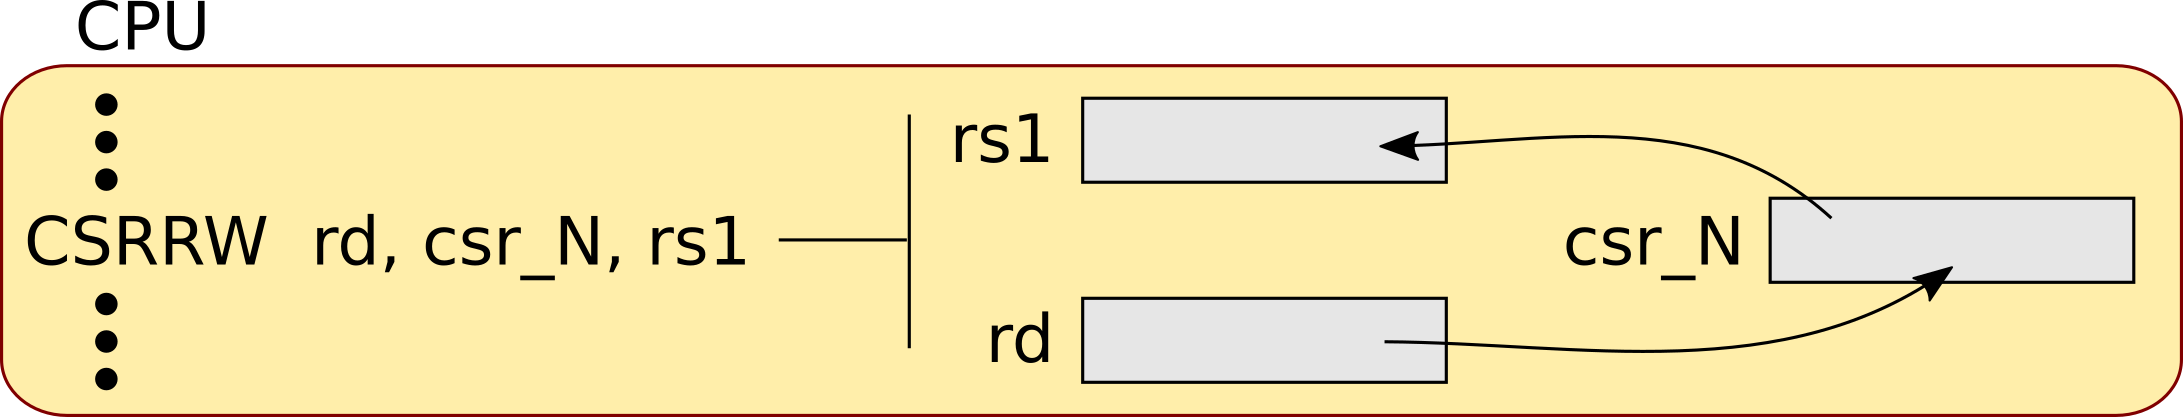
\includegraphics[width=7in]{Figs/CSRRW.png}
    \end{center}

  \end{minipage}
\end{center}

\clearpage

% ================================================================
% CSRs User-Level

\begin{center}
  {\Huge
    CSRs accessible from User level}

  \vspace*{0.2in}

  \begin{minipage}{9in}\LARGE
    \begin{center}
      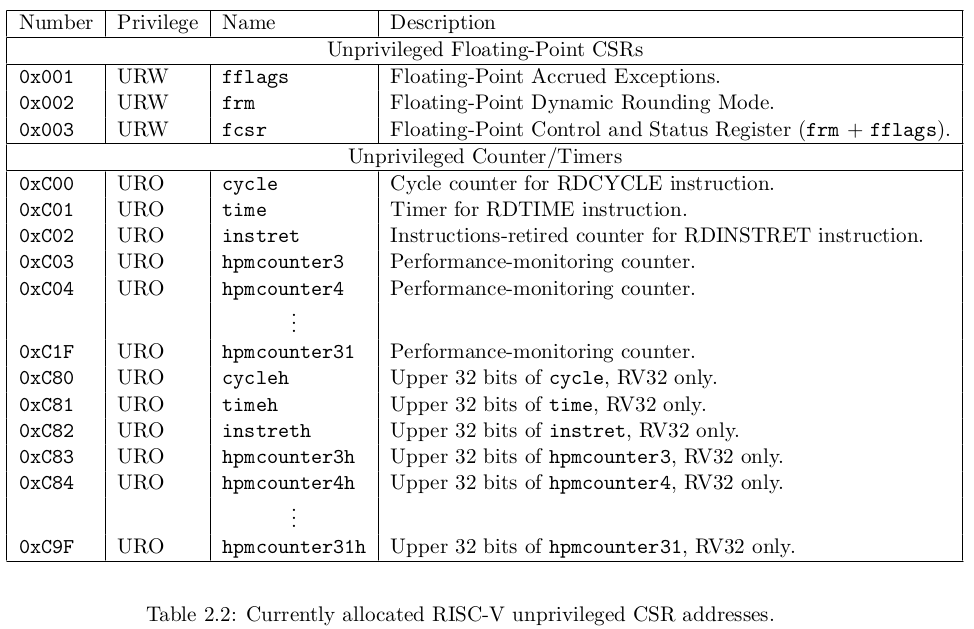
\includegraphics[width=7in]{Figs/CSRs_User_Level.png}
    \end{center}

    \begin{itemize}
    \item CSRs for floating point

    \item CSRs for timing: real-time, cycle, instruction count

    \item CSRs for other performance counters (implementation-defined)
    \end{itemize}
  \end{minipage}

\end{center}

\clearpage

% ================================================================
% CSRs Supervisor-Level

\begin{center}
  {\Huge
    CSRs accessible from Supervisor level}

  \vspace*{0.2in}

  \begin{minipage}{9in}\LARGE
    \begin{center}
      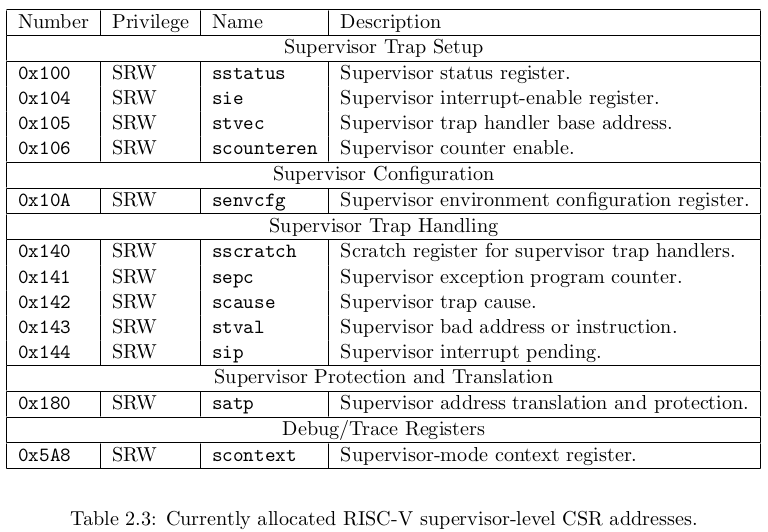
\includegraphics[width=7in]{Figs/CSRs_Supervisor.png}
    \end{center}

    \begin{itemize}
    \item CSRs for handling exceptions (traps and interrupts) at Supervisor level (see later slides)

    \item {\tt satp}: for Virtual memory (see later slides)
    \end{itemize}
  \end{minipage}

\end{center}

\clearpage

% ================================================================
% CSRs Machine-Level

\begin{center}
  {\Huge
    CSRs accessible from Machine level}

  \vspace*{0.2in}

  \begin{minipage}{9in}\LARGE
    \begin{center}
      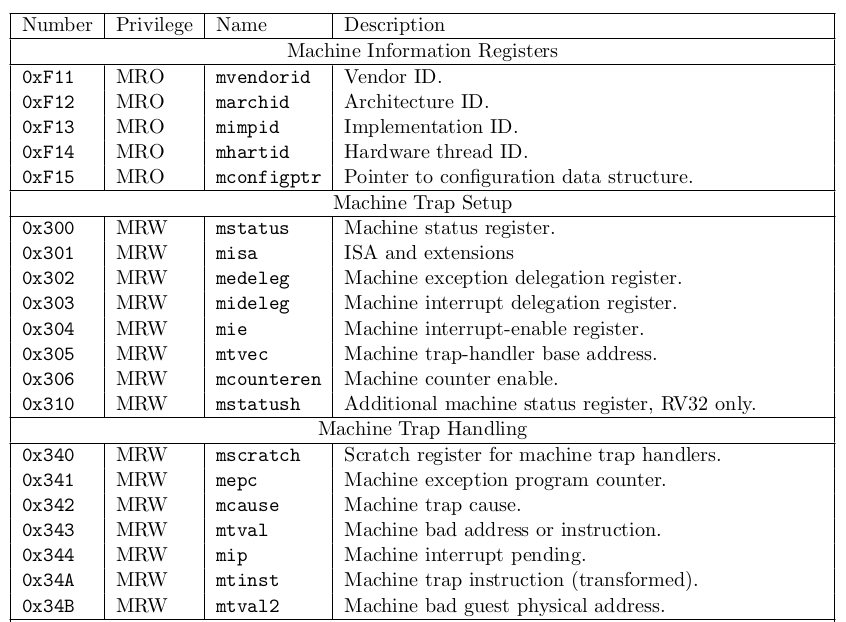
\includegraphics[width=7in]{Figs/CSRs_Machine_Level.png}

      \vspace*{0.1in}

      {\Large (... more ... please consult spec)}
    \end{center}

    \begin{itemize}
    \item CSRs for configuration discovery from software

    \item CSRs for handling exceptions (traps and interrupts) at Machine level (see later slides)
    \end{itemize}
  \end{minipage}

\end{center}

\clearpage

% ================================================================
% Exceptions

\begin{center}
  {\Huge
    Exceptions (Traps and Interrupts)}

  \vspace*{0.2in}

  \begin{minipage}{9.5in}\Large
    \begin{center}
      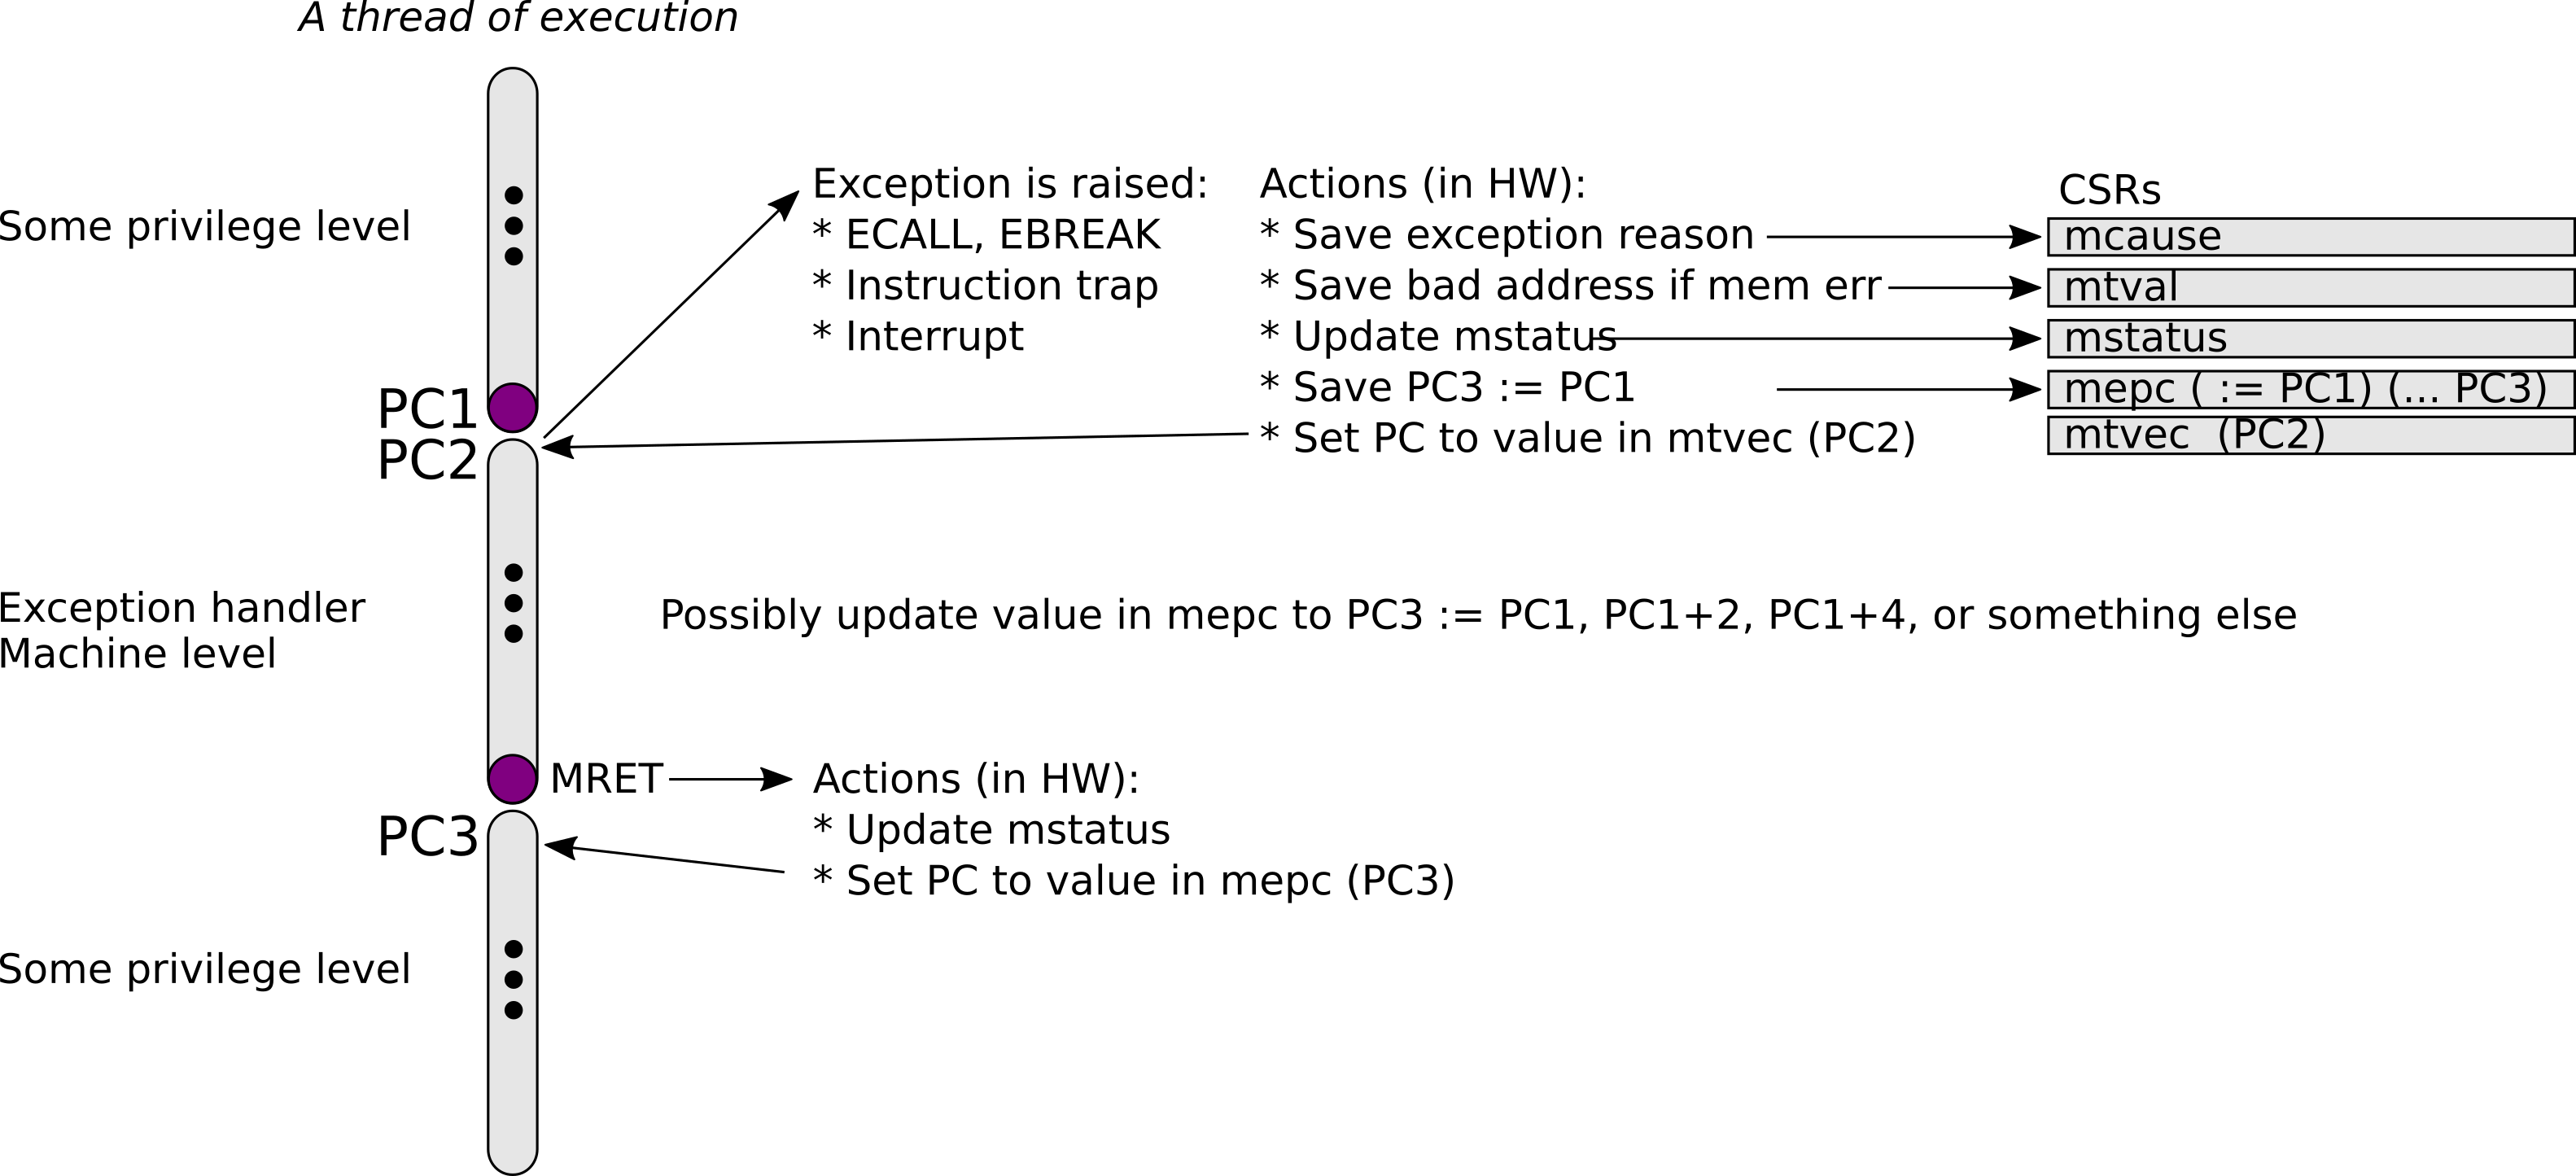
\includegraphics[width=7in]{Figs/Exception_Handling.png}
    \end{center}

    \begin{itemize}
    \item {\tt mtvec} has been pre-loaded before this scenario (by boot-loader, OS, ...)

    \item Saved PC1/+2/+4 depends on whether the instruction needs to
      be retried, and if it is a compressed instruction.

    \item Exception handler can change {\tt mtvec} to some other PC3,
      {\eg} to resume a different thread after the exception.

    \item Any other ``arguments'' and ``results'' are passed in
      registers, according to an ABI/calling convention.

    \item Can be recursive, {\ie} exception handler may itself encounter trap/interrupt.
    \end{itemize}
  \end{minipage}

\end{center}

\clearpage

% ================================================================
% CSR MStatus

\begin{center}
  {\Huge
    CSR MStatus}

  \vspace*{0.3in}

  \begin{minipage}{9.5in}\Large
    \begin{center}
      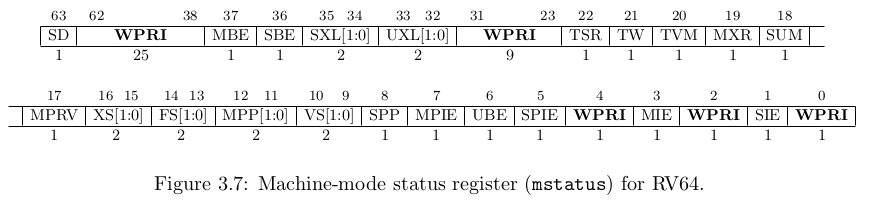
\includegraphics[width=8in]{Figs/CSR_RV64_MStatus.png}
    \end{center}

    \vspace*{0.3in}

    \begin{itemize}
    \item {\tt mstatus} is quite central and critical, and
      manipulation of its bits involves some complexity and subtlety;
      we recommend reading the spec very closely and carefully.

    \item Various bits represent a 2-level ``stack'' (indexed by
      privilege level) that are conceptually pushed on exception entry
      and popped on returns from exceptions (see ``update status'' on
      previous slide).  These include interrupt enable bits (MIE/MPIE,
      SIE/SPIE), previous privilege level (MPP, SPP).

    \item The RV32 version of {\tt mstatus} omits some of the bits.

    \item There is also an {\tt sstatus} CSR at Supervisor level,
      which is similar to, but only a subset of {\tt mstatus}.

    \item Exceptions can be delivered at Machine-level and Supervisor-level privileges.

    \item Exceptions delivered at Machine-level/Supervisor-level can
      be \emph{delegated} to Supervisor-level/User-level (see {\tt
        medeleg} and {\tt mideleg} CSRs).
    \end{itemize}
  \end{minipage}

\end{center}

\clearpage

% ================================================================
% CSR MCause

\begin{center}
  {\Huge
    CSR MCause}
\end{center}

\vspace*{0.2in}

\hmmmm
\begin{minipage}[t]{4in}
  \hmm \\
  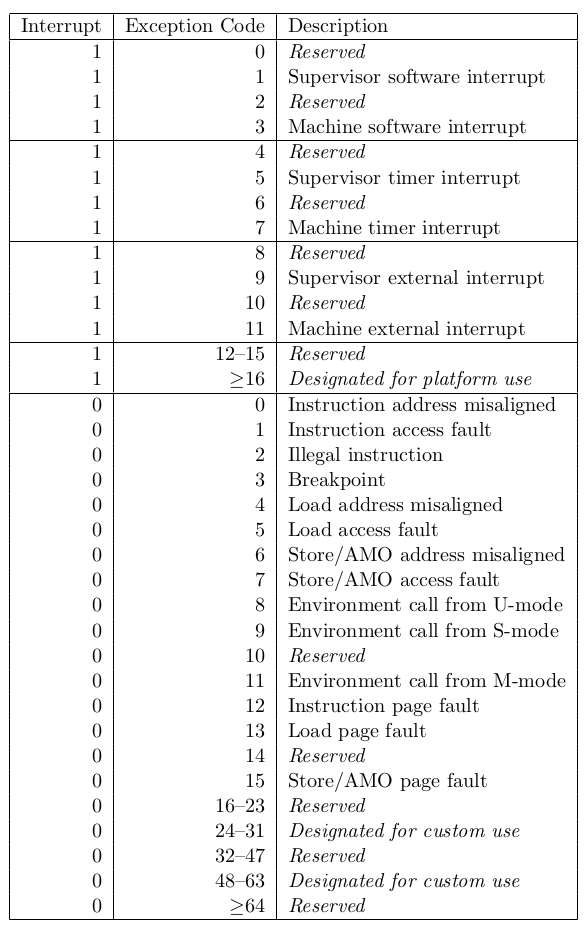
\includegraphics[width=4in]{Figs/CSR_MCause.png}
\end{minipage}
\hm
\begin{minipage}[t]{4.5in}
  \hmm

  \vspace{1in}

  \begin{itemize}\Large
  \item On any exception, the cause is recorded in CSR {\tt mcause}
    during the transfer of control to the exception handler.

  \item Exception-handler code uses {\tt mcause} to discover what kind
    of event caused this exception, using which it can branch to
    event-type-specific handlers.
  \end{itemize}
\end{minipage}

\clearpage

% ================================================================
% CSRs MIP and MIE

\begin{center}
  {\Huge
    CSRs MIP and MIE}

  \vspace*{0.2in}

  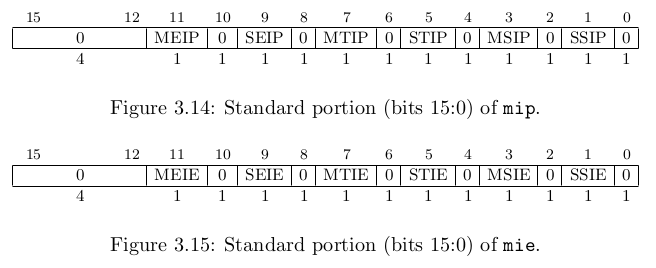
\includegraphics[width=6in]{Figs/CSRs_MIP_MIE.png}

  \vspace*{0.2in}

  \begin{minipage}[t]{9.5in}
    \begin{itemize}\LARGE

    \item Interrupts arrive at a RISC-C hart only via the {\tt mip} CSR.

    \item Both are full-width registers (32b in RV32, 64b in RV64) but
      only the bottom 16 bits have standard definitions.

    \item {\tt mip}: Machine-level register for Interrupts-pending (there
      is also an {\tt sip} for Supervisor level).  The bits can be set
      by various sources of interrupts outside the CPU (see other slides
      on CLIC and PLIC for examples).

    \item Sources can be external devices (``E''), timers (``T'') and
      inter-processor software interrupts (``S'').

    \item {\tt mie}: Machine-level register for Interrupts-enabled (there
      is also an {\tt sie} for Supervisor level).  The CPU can mask-out
      specific source of interrupts by writing 0 to the corresponding
      bit.

    \end{itemize}

    \vspace{0.5in}

  \end{minipage}
\end{center}

\clearpage

% ================================================================
% Sv39 Page Table

\begin{center}
  {\Huge
    Virtual Memory Page Table for Sv39 using CSR {\tt satp}}

  \vspace*{0.1in}

  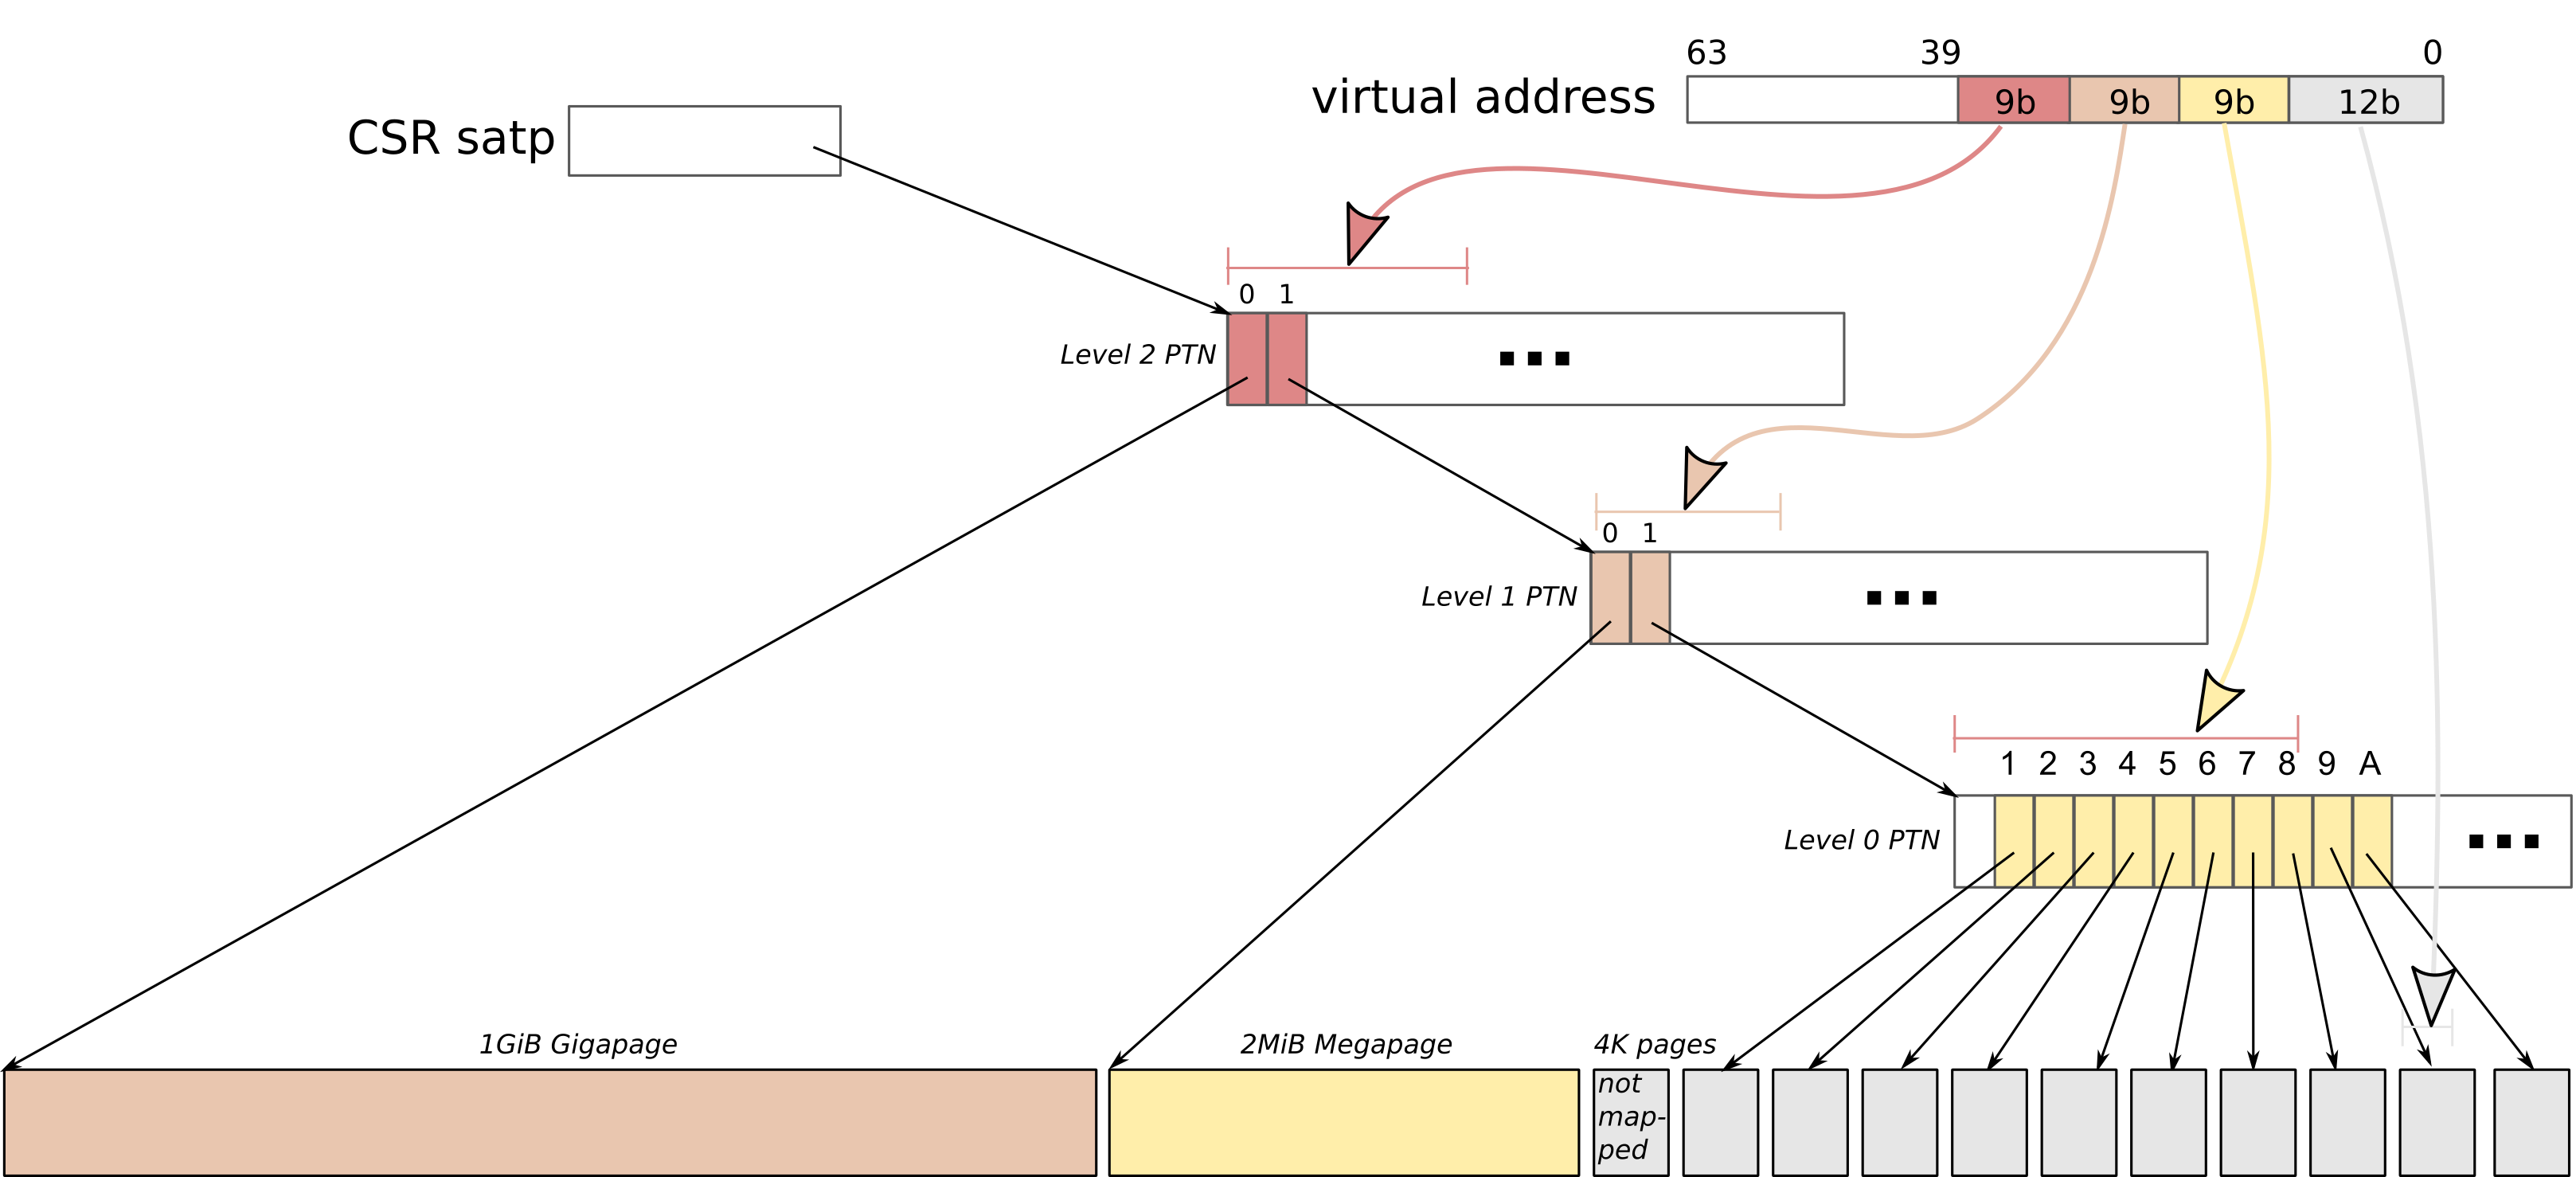
\includegraphics[width=9in]{Figs/VM_Sv39.png}

  \vspace*{0.2in}

  \begin{minipage}[t]{9.5in}
    \begin{itemize}\large

    \item When running in VM mode (indicated by {\tt mstatus} bits,
      privilege level, {\etc}), the PC, and addresses in LD/ST
      instructions are VAs (Virtual Addresses).

    \item CSR {\tt satp} contains a pointer to a 3-level tree.  Each
      node in the tree is a \emph{PTN} (Page Table Node), an aligned
      4KiB block containing 512 \emph{PTEs} (Page Table Entries, each
      64b).  Bits in the PTE indicate whether it is invalid, a leaf
      (pointing to a data page), or a pointer to the next-level node.

    \item Leaves at level 2 point at 1GiB naturally aligned ``gigapages'';
      leaves at level 1 point at 2MiB naturally aligned ``megapages'';
      leaves at level 0 point at 4KiB naturally aligned ``pages'';

    \item Sv39 addresses have 39 bits. 9-bit fields are used to index
      a PTE in a PTN, and the 12 LSBs to index a byte in a page.

      \item If a VA$\rightarrow$PA translation fails (encounter
        invalid PTE, protection failure, ...) it raises a \emph{page
        fault} exception or an \emph{access fault} exception, which is
        handled in the usual way (see ``Exceptions'' slide earlier).
    \end{itemize}
  \end{minipage}
\end{center}

\clearpage

% ===================================================================
% Sv39 Page Table: details

\begin{center}
  {\Huge
    Standard Virtual Memory Schemes}

  \vspace*{1in}

  \begin{minipage}[t]{9in}
    \begin{itemize}\Large
 
    \item The Privileged ISA for RV32 defines one standard Virtual Memory scheme: Sv32.

    \item The Privileged ISA for RV64 defines three standard Virtual
      Memory scheme: Sv39, Sv48 and Sv57.

    \item It is a choice for an implementation as to \emph{how}
      VA$\rightarrow$PA translation is implemented: in hardware or
      firmware or trap-handlers, whether it uses accelerators like
      TLBs (Translation Look-aside Buffers) {\etc} The SFENCE.VMA
      instruction is available to synchronize updates to
      address-translation hardware.

    \end{itemize}
  \end{minipage}
\end{center}

\clearpage

% ================================================================
% Common System Components

\begin{center}
  {\Huge
    Common System Components accompanying RISC-V Cores}

  \vspace*{1in}

  \fbox{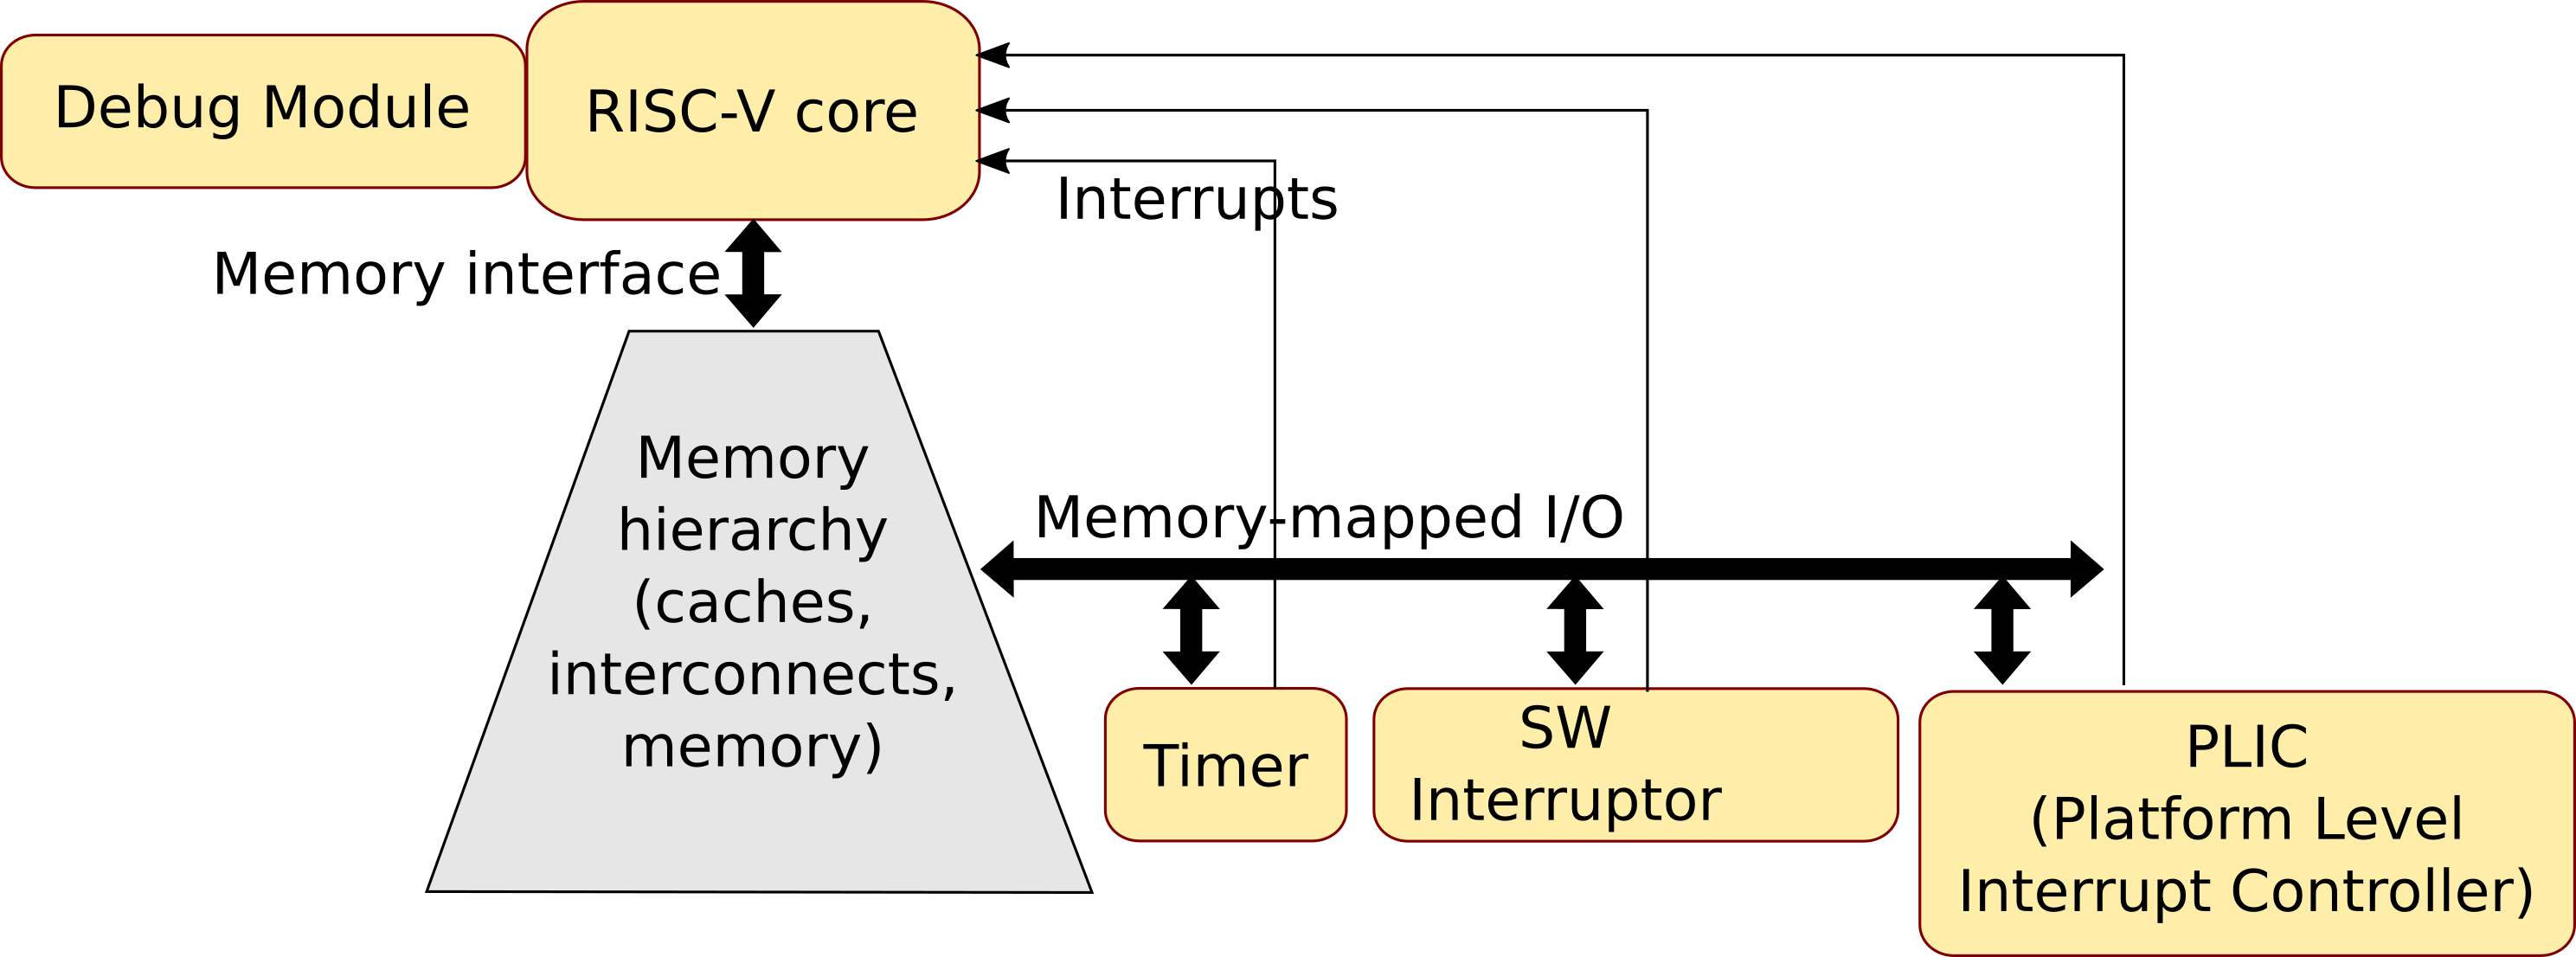
\includegraphics[width=7in]{Figs/Common_System_Components.png}}

  \vspace*{0.5in}

  {\LARGE Each is described in more detail in the following slides.}

\end{center}

\clearpage

% ================================================================
% Timer

\begin{center}
  {\Huge
    Timer: Common System Component accompanying RISC-V Cores}

  \vspace*{0.2in}

  \fbox{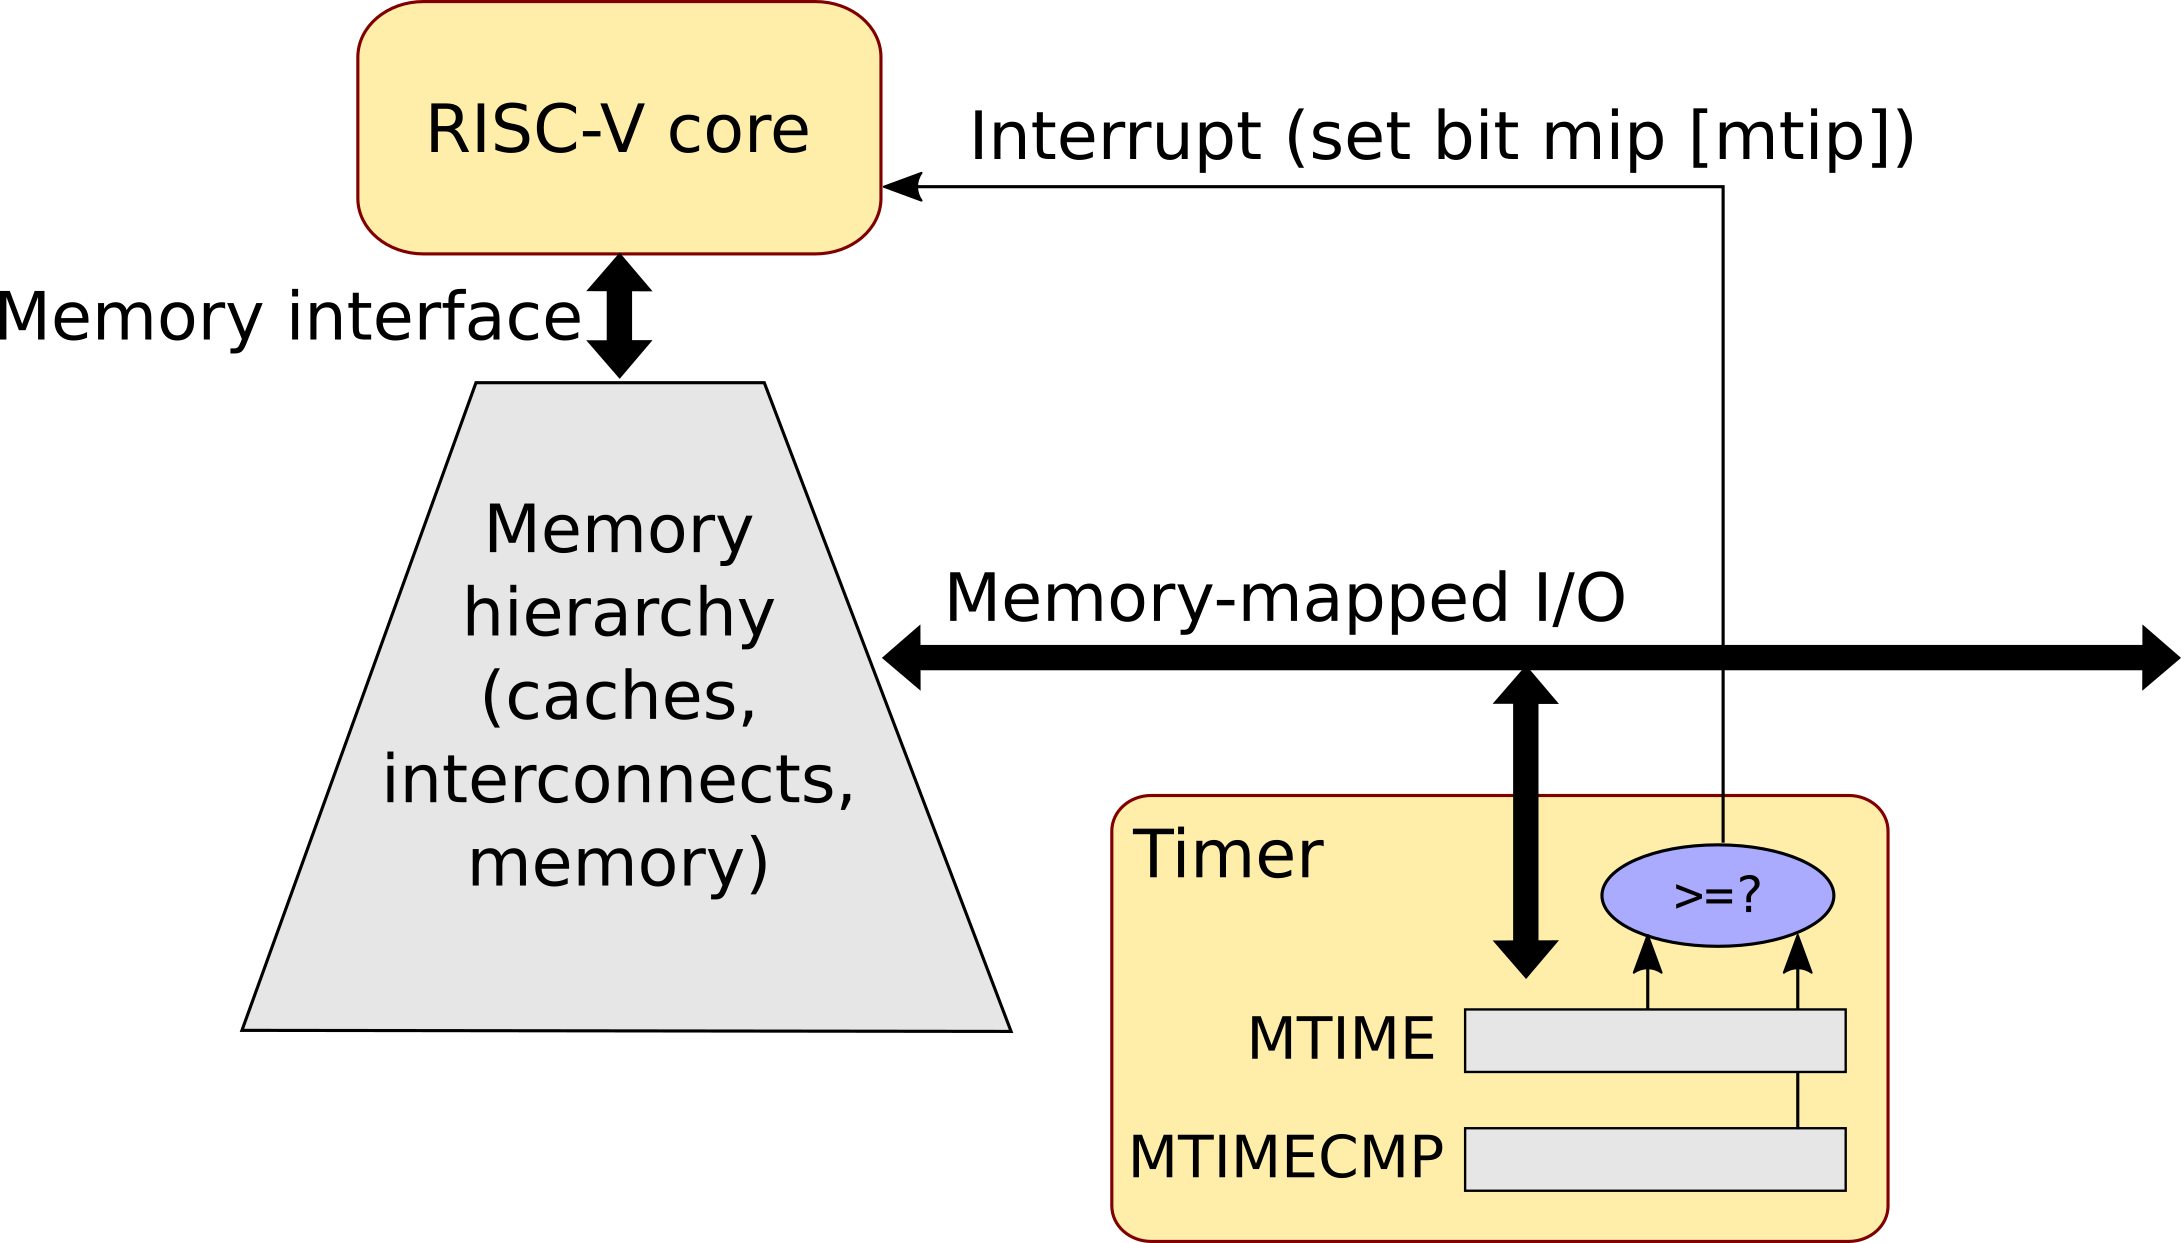
\includegraphics[width=6in]{Figs/Timer.png}}

  \vspace*{0.3in}

  \begin{minipage}[t]{9in}
    \begin{itemize}\LARGE
    \item For SW to measure real-time, and for real-time timer interupts
    \item Contains two memory-mapped registers, MTIME and MTIMECMP
    \item MTIME ticks upwards constantly.
    \item Timer Interrupts: typical usage:
      \begin{itemize}
      \item CPU reads MTIME (let's call it $t$)
      \item CPU writes $t + \delta$ in MTIMECMP
      \item When MTIME ticks up by $\delta$ (so MTIME $\geq$
        MTIMECMP), delivers an interrupt to CSR MIP at the MTIP bit position.
      \end{itemize}
    \end{itemize}
  \end{minipage}
\end{center}

\clearpage

% ================================================================
% SW Interruptor

\begin{center}
  {\Huge
    SW Interruptor: Common System Component accompanying RISC-V Cores}

  \vspace*{0.2in}

  \fbox{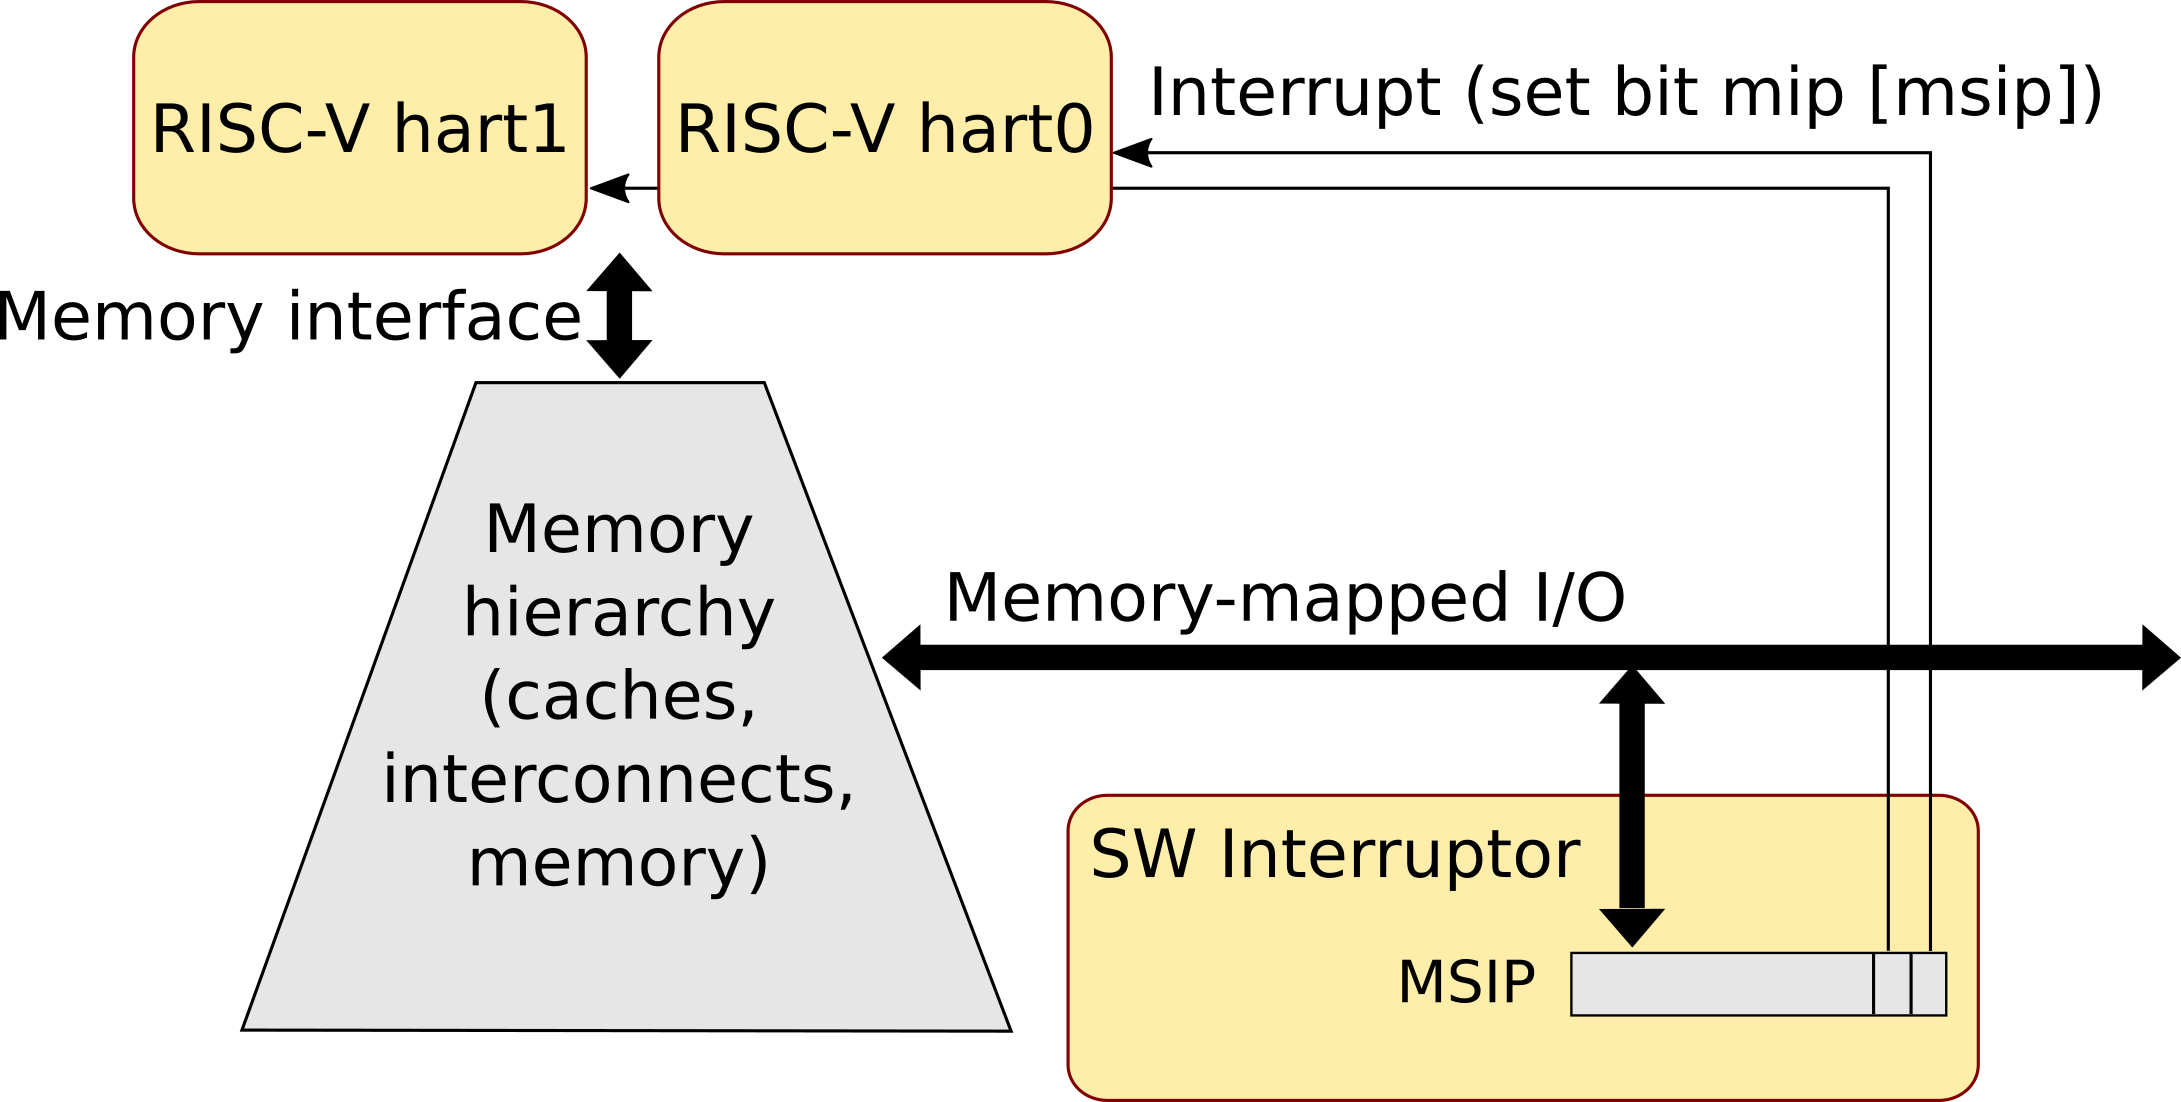
\includegraphics[width=6in]{Figs/SW_Interruptor.png}}

  \vspace*{0.3in}

  \begin{minipage}[t]{9in}
    \begin{itemize}\LARGE
    \item For a hart to deliver a ``sofware interrupt'' to another (or same) hart.
    \item Illustration shows only two harts, but there could be more (multicore).
    \item Contains one memory-mapped register, MSIP
    \item SW Interruptor: typical usage:
      \begin{itemize}
      \item Hart $I$ writes MSIP [$J$] to deliver a SW interrupt to hart $J$
      \item MSIP [$J$] is connected to the CSR MIP at the MSIP bit position (in core $J$).
      \end{itemize}
    \end{itemize}
  \end{minipage}
\end{center}

\clearpage

% ================================================================
% PLIC

\begin{center}
  {\Huge
    PLIC: Common System Component accompanying RISC-V Cores}

  \vspace*{0.5in}

  \fbox{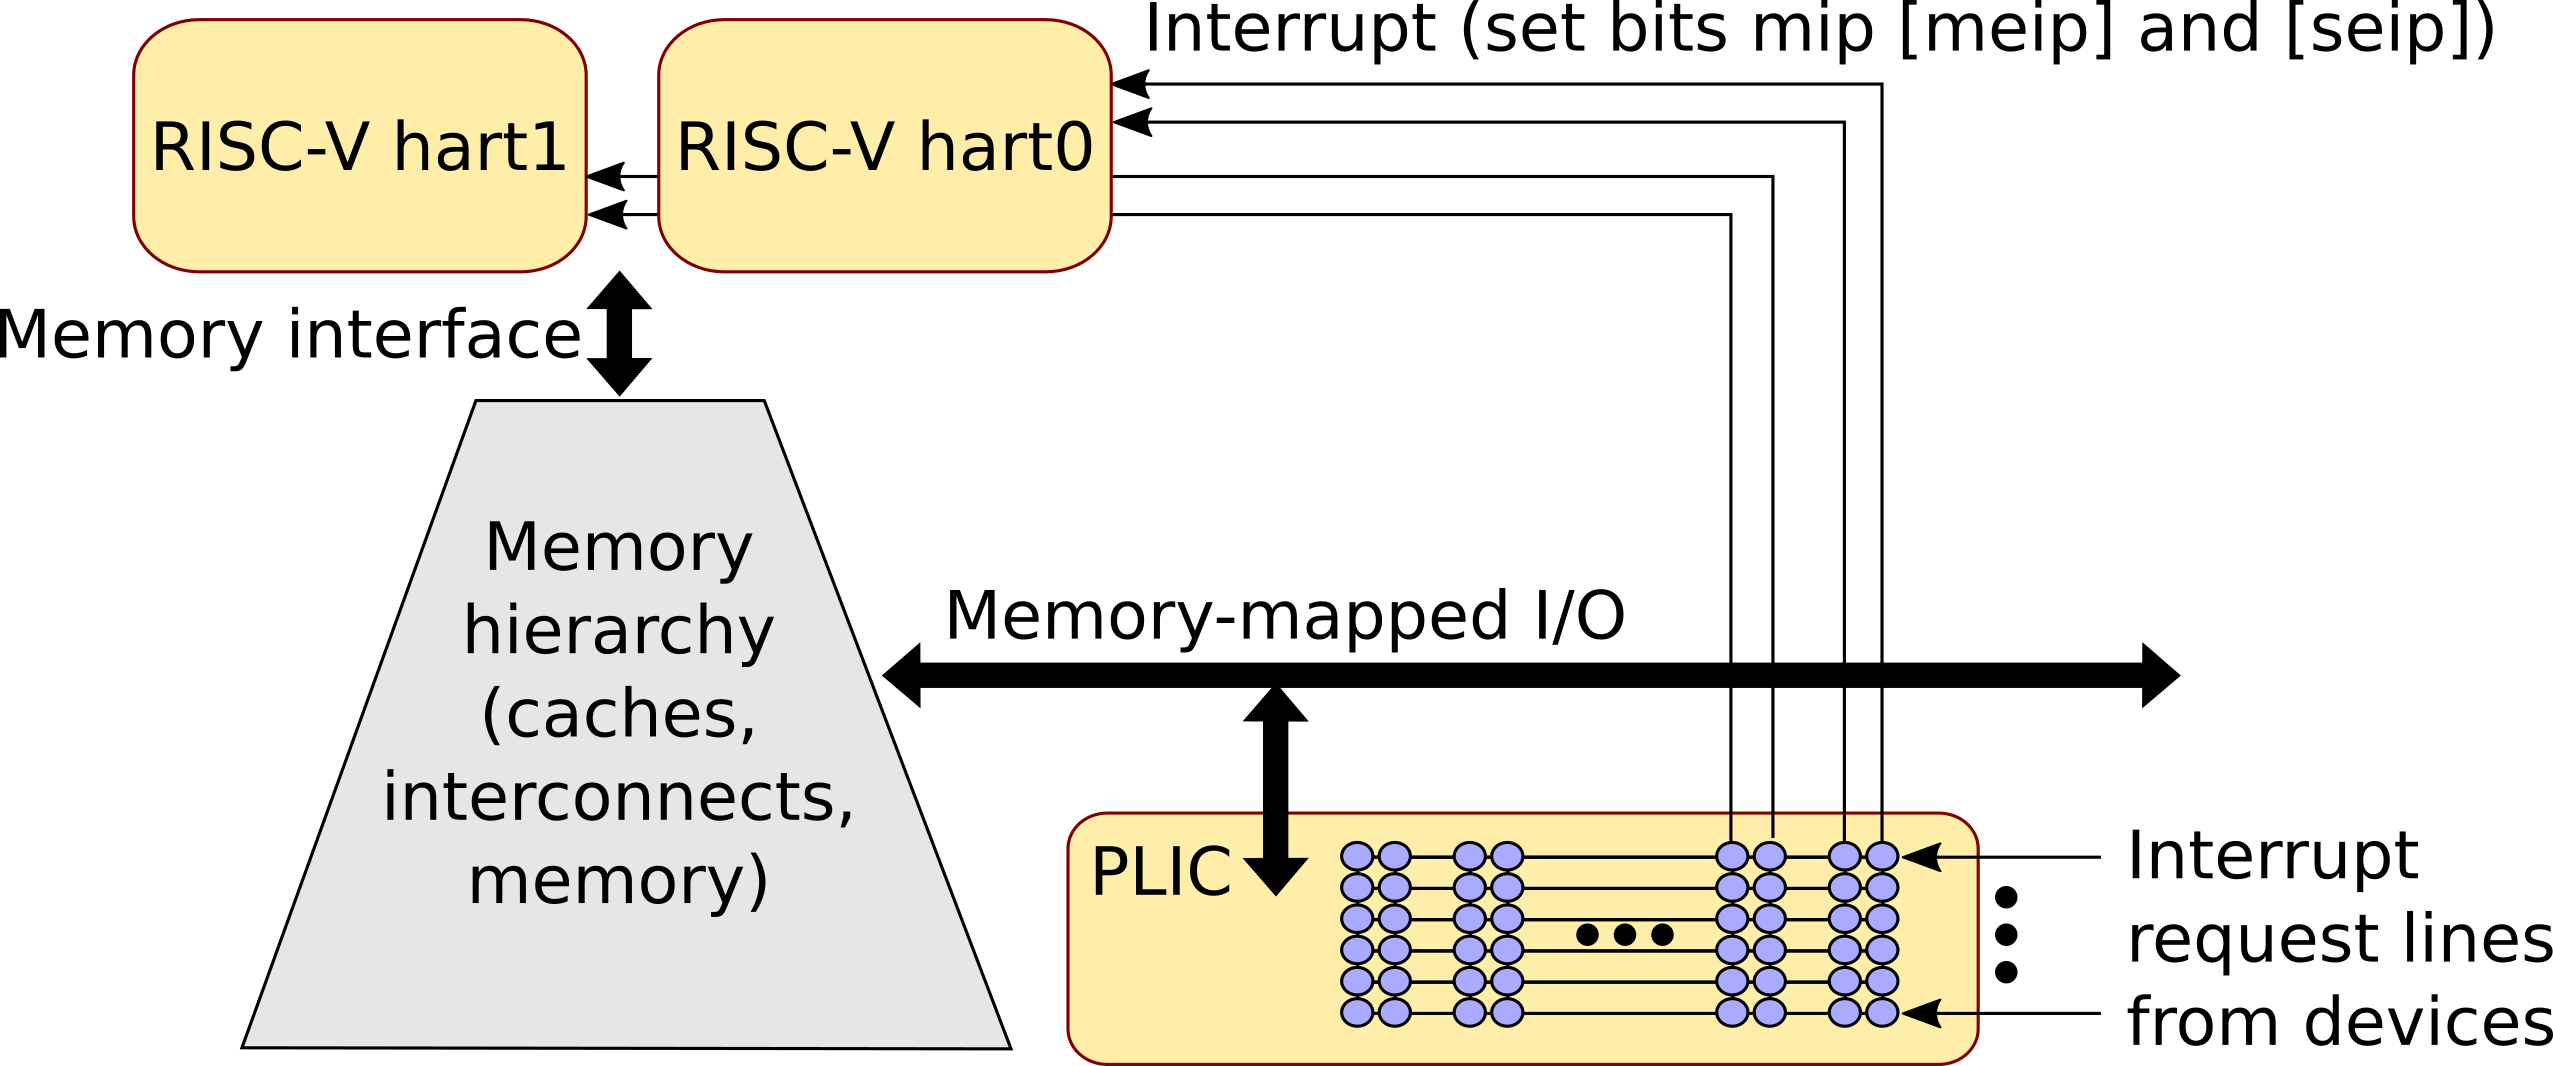
\includegraphics[width=6in]{Figs/PLIC.png}}

  \vspace*{0.5in}

  \begin{minipage}[t]{9in}
    \begin{itemize}\LARGE

    \item Conceptually a matrix connecting an interrupt request line
      from a device to MIP[MEIP] or MIP[SEIP] of any of multiple harts.

    \item Illustration shows only two harts, but there could be more (multicore).

    \item Matrix nodes can be programmed by MMIO from cores to
      configure connectivity, priority, arbitration, interrupt masks, {\etc}

    \item A device interrupt can connect to multiple cores; PLIC has
      facilities for a core to ``claim'' an interrupt atomically.
    \end{itemize}
  \end{minipage}
\end{center}

\clearpage

% ================================================================
% Debug Module

\begin{center}
  {\Huge
    Debug Module: Common System Component accompanying RISC-V Cores}

  \vspace*{0.5in}

  \fbox{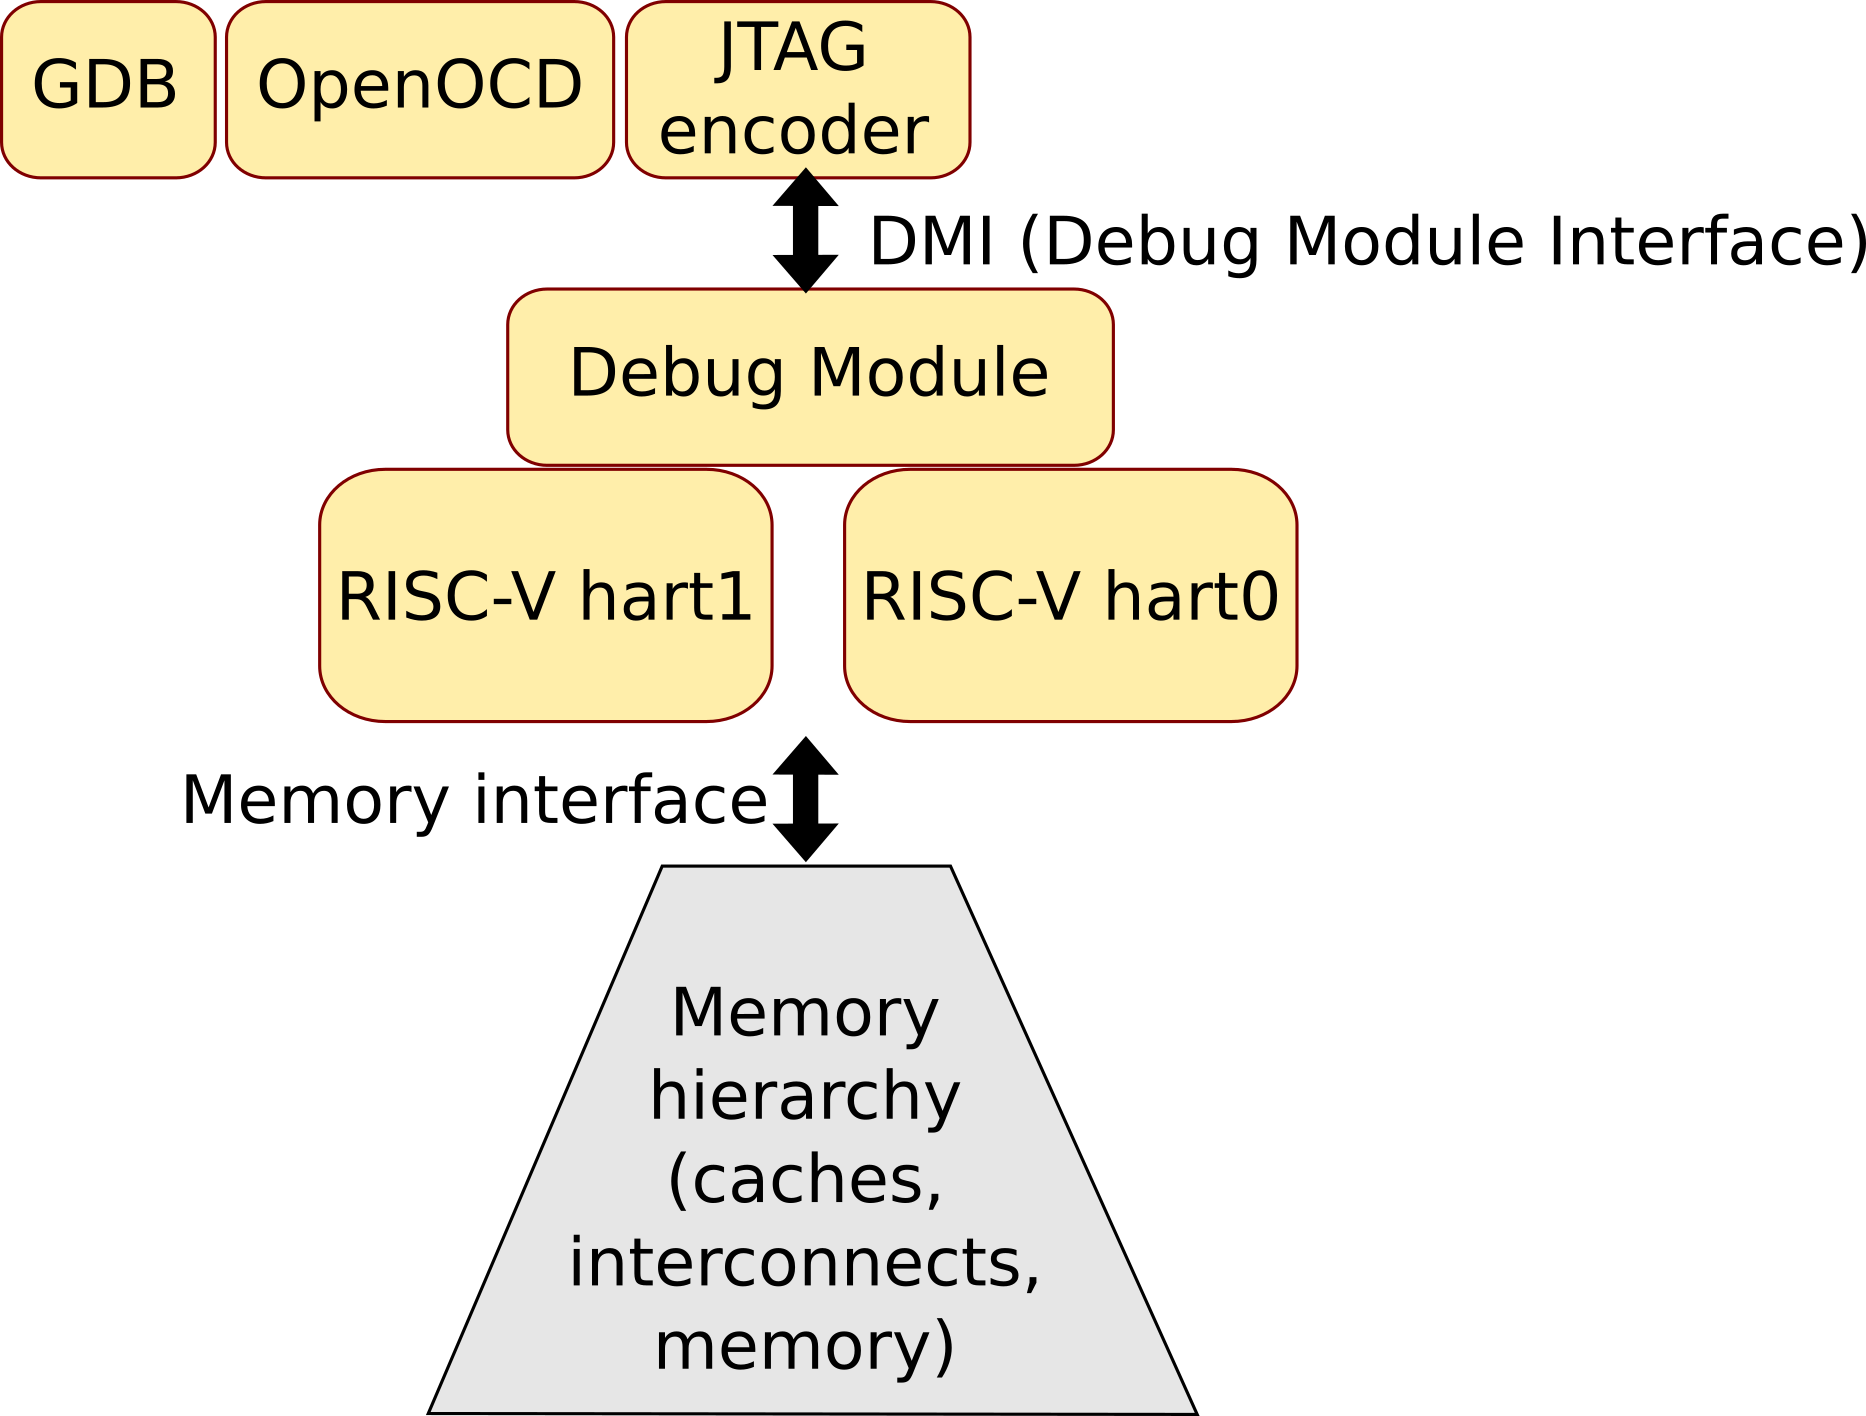
\includegraphics[width=4in]{Figs/Debug_Module.png}}

  \vspace*{0.5in}

  \begin{minipage}[t]{9in}
    \begin{itemize}\LARGE

    \item A RISC-V Debug Module is a HW module closely connected to
      multiple harts.  Can control them individually and collectively.

    \item Functions: Reset hart, read/write registers and CSRs,
      read/write memory, stop/start/continue/single-step, set
      breakpoints, set watchpoints, ...

    \item Is controlled through a standard Debug Module Interface
      (DMI).

    \item Open-source code exists to JTAG-encode the DMI interface.

    \item Can connect from standard OpenOCD (Open On Chip Debugger) and GDB.
    \end{itemize}
  \end{minipage}
\end{center}

\clearpage

% ================================================================
% RISC-V Software

\begin{center}
  {\Huge
    A Note about the RISC-V Software Ecosystem}

  \vspace*{1in}

  \begin{minipage}{9in}\LARGE
    \begin{itemize}
    \item Mature: GNU toolchain (gcc, gdb, ...)
    \item Mature: Linux, FreeRTOS, seL4, ...
    \item Hundreds/thousands of other porting efforts underway; ecosystem grows every day.
    \end{itemize}
  \end{minipage}

\end{center}

\clearpage

% ================================================================

\end{document}
